% Options for packages loaded elsewhere
\PassOptionsToPackage{unicode}{hyperref}
\PassOptionsToPackage{hyphens}{url}
%
\documentclass[
]{article}
\usepackage{amsmath,amssymb}
\usepackage{lmodern}
\usepackage{iftex}
\ifPDFTeX
  \usepackage[T1]{fontenc}
  \usepackage[utf8]{inputenc}
  \usepackage{textcomp} % provide euro and other symbols
\else % if luatex or xetex
  \usepackage{unicode-math}
  \defaultfontfeatures{Scale=MatchLowercase}
  \defaultfontfeatures[\rmfamily]{Ligatures=TeX,Scale=1}
\fi
% Use upquote if available, for straight quotes in verbatim environments
\IfFileExists{upquote.sty}{\usepackage{upquote}}{}
\IfFileExists{microtype.sty}{% use microtype if available
  \usepackage[]{microtype}
  \UseMicrotypeSet[protrusion]{basicmath} % disable protrusion for tt fonts
}{}
\makeatletter
\@ifundefined{KOMAClassName}{% if non-KOMA class
  \IfFileExists{parskip.sty}{%
    \usepackage{parskip}
  }{% else
    \setlength{\parindent}{0pt}
    \setlength{\parskip}{6pt plus 2pt minus 1pt}}
}{% if KOMA class
  \KOMAoptions{parskip=half}}
\makeatother
\usepackage{xcolor}
\usepackage[margin=1in]{geometry}
\usepackage{graphicx}
\makeatletter
\def\maxwidth{\ifdim\Gin@nat@width>\linewidth\linewidth\else\Gin@nat@width\fi}
\def\maxheight{\ifdim\Gin@nat@height>\textheight\textheight\else\Gin@nat@height\fi}
\makeatother
% Scale images if necessary, so that they will not overflow the page
% margins by default, and it is still possible to overwrite the defaults
% using explicit options in \includegraphics[width, height, ...]{}
\setkeys{Gin}{width=\maxwidth,height=\maxheight,keepaspectratio}
% Set default figure placement to htbp
\makeatletter
\def\fps@figure{htbp}
\makeatother
\setlength{\emergencystretch}{3em} % prevent overfull lines
\providecommand{\tightlist}{%
  \setlength{\itemsep}{0pt}\setlength{\parskip}{0pt}}
\setcounter{secnumdepth}{-\maxdimen} % remove section numbering
\newlength{\cslhangindent}
\setlength{\cslhangindent}{1.5em}
\newlength{\csllabelwidth}
\setlength{\csllabelwidth}{3em}
\newlength{\cslentryspacingunit} % times entry-spacing
\setlength{\cslentryspacingunit}{\parskip}
\newenvironment{CSLReferences}[2] % #1 hanging-ident, #2 entry spacing
 {% don't indent paragraphs
  \setlength{\parindent}{0pt}
  % turn on hanging indent if param 1 is 1
  \ifodd #1
  \let\oldpar\par
  \def\par{\hangindent=\cslhangindent\oldpar}
  \fi
  % set entry spacing
  \setlength{\parskip}{#2\cslentryspacingunit}
 }%
 {}
\usepackage{calc}
\newcommand{\CSLBlock}[1]{#1\hfill\break}
\newcommand{\CSLLeftMargin}[1]{\parbox[t]{\csllabelwidth}{#1}}
\newcommand{\CSLRightInline}[1]{\parbox[t]{\linewidth - \csllabelwidth}{#1}\break}
\newcommand{\CSLIndent}[1]{\hspace{\cslhangindent}#1}
\usepackage{lineno}
\linenumbers
\usepackage{setspace}\doublespacing
\usepackage{gensymb}
\geometry{verbose,letterpaper,tmargin=2.54cm,bmargin=2.54cm,lmargin=2.54cm,rmargin=2.54cm}
\usepackage[nomarkers,figuresonly]{endfloat}
\usepackage{float}
\ifLuaTeX
  \usepackage{selnolig}  % disable illegal ligatures
\fi
\IfFileExists{bookmark.sty}{\usepackage{bookmark}}{\usepackage{hyperref}}
\IfFileExists{xurl.sty}{\usepackage{xurl}}{} % add URL line breaks if available
\urlstyle{same} % disable monospaced font for URLs
\hypersetup{
  hidelinks,
  pdfcreator={LaTeX via pandoc}}

\author{}
\date{\vspace{-2.5em}}

\begin{document}

\hypertarget{quantifying-impacts-of-an-environmental-intervention-using-environmental-dna}{%
\subsection{Quantifying Impacts of an Environmental Intervention Using
Environmental
DNA}\label{quantifying-impacts-of-an-environmental-intervention-using-environmental-dna}}

Elizabeth Andruszkiewicz Allan\(^{1*\dagger}\), Ryan P. Kelly\(^{1*}\),
Erin R. D'Agnese\(^{1}\), Maya N. Garber-Yonts\(^{1}\), Megan R.
Shaffer\(^{1}\), Zachary J. Gold\(^{2}\), Andrew O. Shelton\(^{2}\)

\(^{1}\) University of Washington, School of Marine and Environmental
Affairs, 3737 Brooklyn Ave NE, Seattle, WA 98105, U.S.A.

\(^2\)Conservation Biology Division, Northwest Fisheries Science Center,
National Marine Fisheries Service, National Oceanic and Atmospheric
Administration, 2725 Montlake Blvd. E, Seattle, WA 98112, U.S.A.

\vspace{1em}

\(^{*}\) Authors contributed equally to this work.

\(^{\dagger}\) Corresponding author:
\href{mailto:eallan@uw.edu}{\nolinkurl{eallan@uw.edu}} \vspace{1em}

For submission to: \textit{Ecological Applications} \newline Manuscript
type: Article \newline Open Research Statement: Data are provided as
private-for-peer review (shared privately or publicly on a repository).
The repository for code can be found at:
\url{https://github.com/eandrusz/quantitative_salmon_culverts.git}
\newline \textit{Keywords: environmental DNA, quantitative metabarcoding, environmental impact assessments, salmon, culvert}

\newpage

\hypertarget{abstract}{%
\subsection{Abstract}\label{abstract}}

Environmental laws around the world require some version of an
environmental impact assessment surrounding construction projects and
other discrete instances of human development. Information requirements
for these assessments vary by jurisdiction, but nearly all require an
analysis of the biological elements of affected ecosystems.
Amplicon-sequencing - also called metabarcoding - of environmental DNA
(eDNA) has made it possible to sample and amplify the genetic material
of many species present in those environments, providing a tractable,
powerful, and increasingly common way of doing environmental impact
analysis for development projects. Here, we analyze a 12-month
time-series of water samples taken before, during, and after a culvert
removal project in a salmonid-bearing freshwater stream. We use an
asymmetrical Before-After-Control-Impact (BACI) design with multiple
control streams to develop a robust background expectation against which
to evaluate the impact of this discrete environmental intervention in
the treatment stream. We generate calibrated, quantitative metabarcoding
data from amplifying the 12s MiFish mtDNA locus and complementary
species-specific quantitative PCR data to yield multi-species estimates
of absolute eDNA concentrations across time, creeks, and sampling
stations. We then use a hierarchical Bayesian time-series model to
reveal patterns of eDNA concentrations over time, and to estimate the
effects of the culvert removal on salmonids in the treatment creek. We
focus our analysis on four common salmonid species: cutthroat trout
(\emph{Oncorhynchus clarkii}), coho salmon (\emph{O. kisutch}),
rainbow/steelhead trout (\emph{O. mykiss}), and sockeye/kokanee salmon
(\emph{O. nerka}). After accounting for temporal variability common to
the sampled creeks, we find only transient effects on these species
during the several months after construction. In the context of billions
of dollars of court-mandated road culvert replacements taking place in
Washington State, USA, our results suggest that culvert replacement can
be conducted with only minimal impact of construction to key species of
management concern. Furthermore, eDNA methods can be an effective and
efficient approach for monitoring hundreds of culverts to prioritize
culverts that are required to be replaced. More broadly, we demonstrate
a rigorous, quantitative method for environmental impact reporting using
eDNA that is widely applicable in environments worldwide.

\newpage

\hypertarget{introduction}{%
\subsection{Introduction}\label{introduction}}

At present, it remains difficult to comprehensively measure the
environmental impacts of discrete human activities, despite such
assessment often being required by law. Within the United States, both
state and federal laws often require a form of environmental-impact
assessment for medium- to large-scale projects (i.e., those that might
have a significant impact on the environment) (Morgan 2012). Outside the
US, many nations have their own versions of these same laws.
Specifically when measuring impacts on aquatic ecosystems, assessments
generally are based on literature reviews or field measurements of key
species selected beforehand (Rubin et al. 2017). These traditional
methods are often expensive, rely on just a few species, and are limited
in spatial and temporal coverage (Martin et al. 2012). Moreover, they
often lack pre-project monitoring and any or sufficient post-project
monitoring, given that the goals of a development project normally focus
on construction itself and funding is often extremely limited. For
example, a recent literature review of stream restoration projects cited
that more than half of projects evaluated (62\%) had no pre-project
monitoring and only sampled once per year (for before, during, and
post-project sampling) (Rubin et al. 2017). Thus, current assessment
efforts relying on traditional survey methods often fall short in
documenting and quantifying environmental impacts.

A key difficulty in conducting ecosystem assessments is that there is no
one way to survey the world and just ``see what is there.'' All methods
of environmental sampling are biased as they capture a selective portion
of the biodiversity present (Rubin et al. 2017). Net samples for fish,
for example, fail to capture species too small or too large to be caught
in the net. Environmental DNA (eDNA), however, comes as close to this
goal as any method yet developed: a sample of water, soil, or even air,
contains the genetic traces of many thousands of species, from microbes
to whales. Sequencing eDNA is therefore a means of surveying many
species in a consistent and scalable way (Taberlet et al. 2012, Thomsen
and Willerslev 2015). Environmental assessments have begun to make use
of eDNA for such work around the world (Muha et al. 2017, Duda et al.
2021, Klein et al. 2022, Maasri et al. 2022, Moss et al. 2022), but are
not yet common practice. Surveying the world by eDNA has long been
commonplace in microbial ecology (Ogram et al. 1987, Rondon et al. 2000,
Turnbaugh et al. 2007) but has recently become popular for
characterizing eukaryotic communities (Taberlet et al. 2012, Kelly et
al. 2014, De Vargas et al. 2015, Port et al. 2015, Valentini et al.
2016, Stat et al. 2017). Techniques generally include an amplification
step such as quantitative PCR, digital or digital-droplet PCR, or
traditional PCR from mixed templates followed by high-throughput
sequencing (Ruppert et al. 2019). This last technique is known as eDNA
metabarcoding.

In a metabarcoding approach, broad-spectrum PCR primers identify
hundreds or thousands of taxa across a very wide diversity of the tree
of the life (e.g., Leray et al. (2013)), but nevertheless the absence of
a taxon from a sequenced sample does not indicate the absence of that
taxon from the environment but rather that the taxon failed to amplify
(Shelton et al. 2016, Kelly et al. 2019, Buxton et al. 2021). In
virtually all comparisons, metabarcoding recovers far more taxa than any
other sampling method (Port et al. 2015, Kelly et al. 2017, Seymour et
al. 2021). However, we expect results from metabarcoding to differ
dramatically from non-PCR based sampling methods due to the fundamental
differences in sampling genetic waste as opposed to whole organisms.
Furthermore, eDNA analyses rely on several laboratory processes,
including PCR amplification, all of which contribute to complicating the
interpretation of results (see Shelton et al. (2016) and Kelly et al.
(2019)). Specifically, PCR amplification is an exponential process for
which the efficiency varies across species and primer set (Gloor et al.
2016). By understanding these differences, we can correct for
taxon-specific biases to yield quantitative estimates of the community
composition prior to PCR (McLaren et al. 2019, Shelton et al. 2022).

After correcting for amplification biases, the resulting dataset is
compositional, revealing the proportions of each species' DNA present in
each sample, but importantly, contains no information about the absolute
abundance of DNA present (Gloor et al. 2016, McLaren et al. 2019,
Silverman et al. 2021, Shelton et al. 2022). We can tie these
proportional estimates to absolute abundances using additional data such
as a quantitative PCR (qPCR) assay for one of the taxa present. Thus, a
single qPCR assay and a single metabarcoding assay can together provide
quantitative estimates of many species as opposed to running as many
qPCR assays as species of interest. Together, we can use these data to
assess changes in eDNA concentrations of species over time, and due to
environmental impacts, such as replacing a culvert under a road.

As a result of a ruling in a federal court (Martinez 2013), Washington
State is under a court-ordered mandate to replace hundreds of culverts
that allow water to pass under roads and highways, costing billions of
dollars. Improperly designed culverts can lead to many negative
consequences for fish, especially anadromous salmon, including habitat
fragmentation, loss of accessibility to spawning and rearing habitat,
and genetic isolation (Price et al. 2010, Frankiewicz et al. 2021).
These impacts on salmonids furthermore violate the sovereign treaty
rights of the region's indigenous tribes to manage their people, land,
and resources (Schmidhauser 1976a). Salmonid species are of cultural and
economic importance to the indigenous peoples of the region, and without
restoration of historic salmon-rearing habitat, the continued decline of
salmonids can lead to not only ecological destruction, but the loss of
cultural and economic viability for many indigenous tribes (Schmidhauser
1976b, Lackey 2003, Long and Lake 2018).

Presently, the prioritization process for replacing culverts preventing
fish passage conducted by the Washington Department of Transportation is
a protocol provided by the Washington Department of Fish and Wildlife,
which includes factors such as the amount of habitat blocked by the
barrier, the types of species blocked by the barrier, and estimated cost
of repair, among other things (Washington Department of Fish and
Wildlife 2019). However, data on fish presence upstream of barriers
(i.e., culverts blocking fish passage) are rare and often not included
in these assessments. Using eDNA as a proxy for fish presence could
provide important data for project prioritization.

Once a culvert has been designated as in need of repair, the intention
is to improve conditions for biota, including migrating fish, but the
construction itself might have a short-term negative effect before the
longer-term improvements are realized. Specifically in culvert
replacements, studies have cited the negative impacts of construction to
include sediment accumulation, removal of vegetation, and blocking flow
and stranding fish (Wellman et al. 2000, Washington Department of Fish
and Wildlife 2019). However, it is unclear how long these effects might
last and if the long-term benefits of the culvert replacement justify
the short-term costs of the construction. These disruptions also
underscore the importance of both properly assessing culverts to
determine if they are blocking fish passage and monitoring after
construction to ensure the replacement actually improved fish passage.

Many studies have attempted to quantify if culverts are barriers to fish
passage and how effective culvert replacements are for fish passage,
either by measuring physical parameters of the culvert and stream after
replacement (Price et al. 2010), or by measuring biological parameters,
including electrofishing (Ogren and Huckins 2015) or utilizing genetic
differentiation from fish tissues (Wood et al. 2018, Nathan et al.
2018). MacPherson et al. (2012) found in a study of over 200 culverts,
that for certain species, including rainbow trout (\emph{O. mykiss}),
culverts were not blocking fish passage despite being deemed blockages.
As for how effective replacements are, Price et al. (2010) found in a
study of \textasciitilde75 culverts that, despite culvert replacement,
about 30\% of the new culverts still remained blockages (by physical
characterization), while Ogren and Huckins (2015) found in a more
in-depth study of just three culverts that after biological sampling
(i.e., electrofishing and macroinvertebrate surveys) 3-5 years after
culvert replacements, the overall biotic integrity was not improved.
Sampling water for eDNA analysis before, during, and post-restoration
can provide valuable information on if the restoration is needed, how
the restoration negatively impacts communities during construction, and
if the restoration efforts did in fact correct the blockage.

Here, we report the results of a year-long eDNA sampling effort before,
during, and after a small construction project in our experimental
creek, assessing the impact of that project on the salmonid species
present. We do so using a combination of metabarcoding (12s mtDNA) and
qPCR to yield estimates of the concentrations of DNA present at each
time point, and we use parallel samples from an additional four control
creeks to develop a causal analysis of changes in these concentrations.
A clear opportunity for policy-relevant eDNA work is in using its power
to survey many species at a time to improve the way we assess the
impacts of human activities. Here, we demonstrate the utility of eDNA
for such assessments.

\hypertarget{methods}{%
\subsection{Methods}\label{methods}}

\hypertarget{site-and-species-selection}{%
\subsubsection{Site and Species
Selection}\label{site-and-species-selection}}

We selected sampling locations based loosely on an asymmetrical BACI
(Before-After-Control-Impact) study design (Underwood 1992, 1994,
Benedetti-Cecchi 2001) to measure the environmental impact of a culvert
replacement using eDNA. We sampled four control creeks, which all had
culverts not under construction, (Figure \ref{fig:map}) at monthly
intervals, both upstream and downstream of each creek's culvert. The
culvert in the treatment creek (Padden) was suspected to be partially
impassible and thus was removed and replaced during the course of the
study; the four control creeks ranged from preventing fish passage
(Barnes and Chuckanut), partially passable (Squalicum), to allowing fish
passage (Portage; see Supplemental Text 1) (Washington Department of
Fish and Wildlife 2019). These creeks were chosen due to their
comparable size, flow, watersheds, and species presumed to be present to
constrain as many ecological variables as possible.

\begin{figure}
\centering
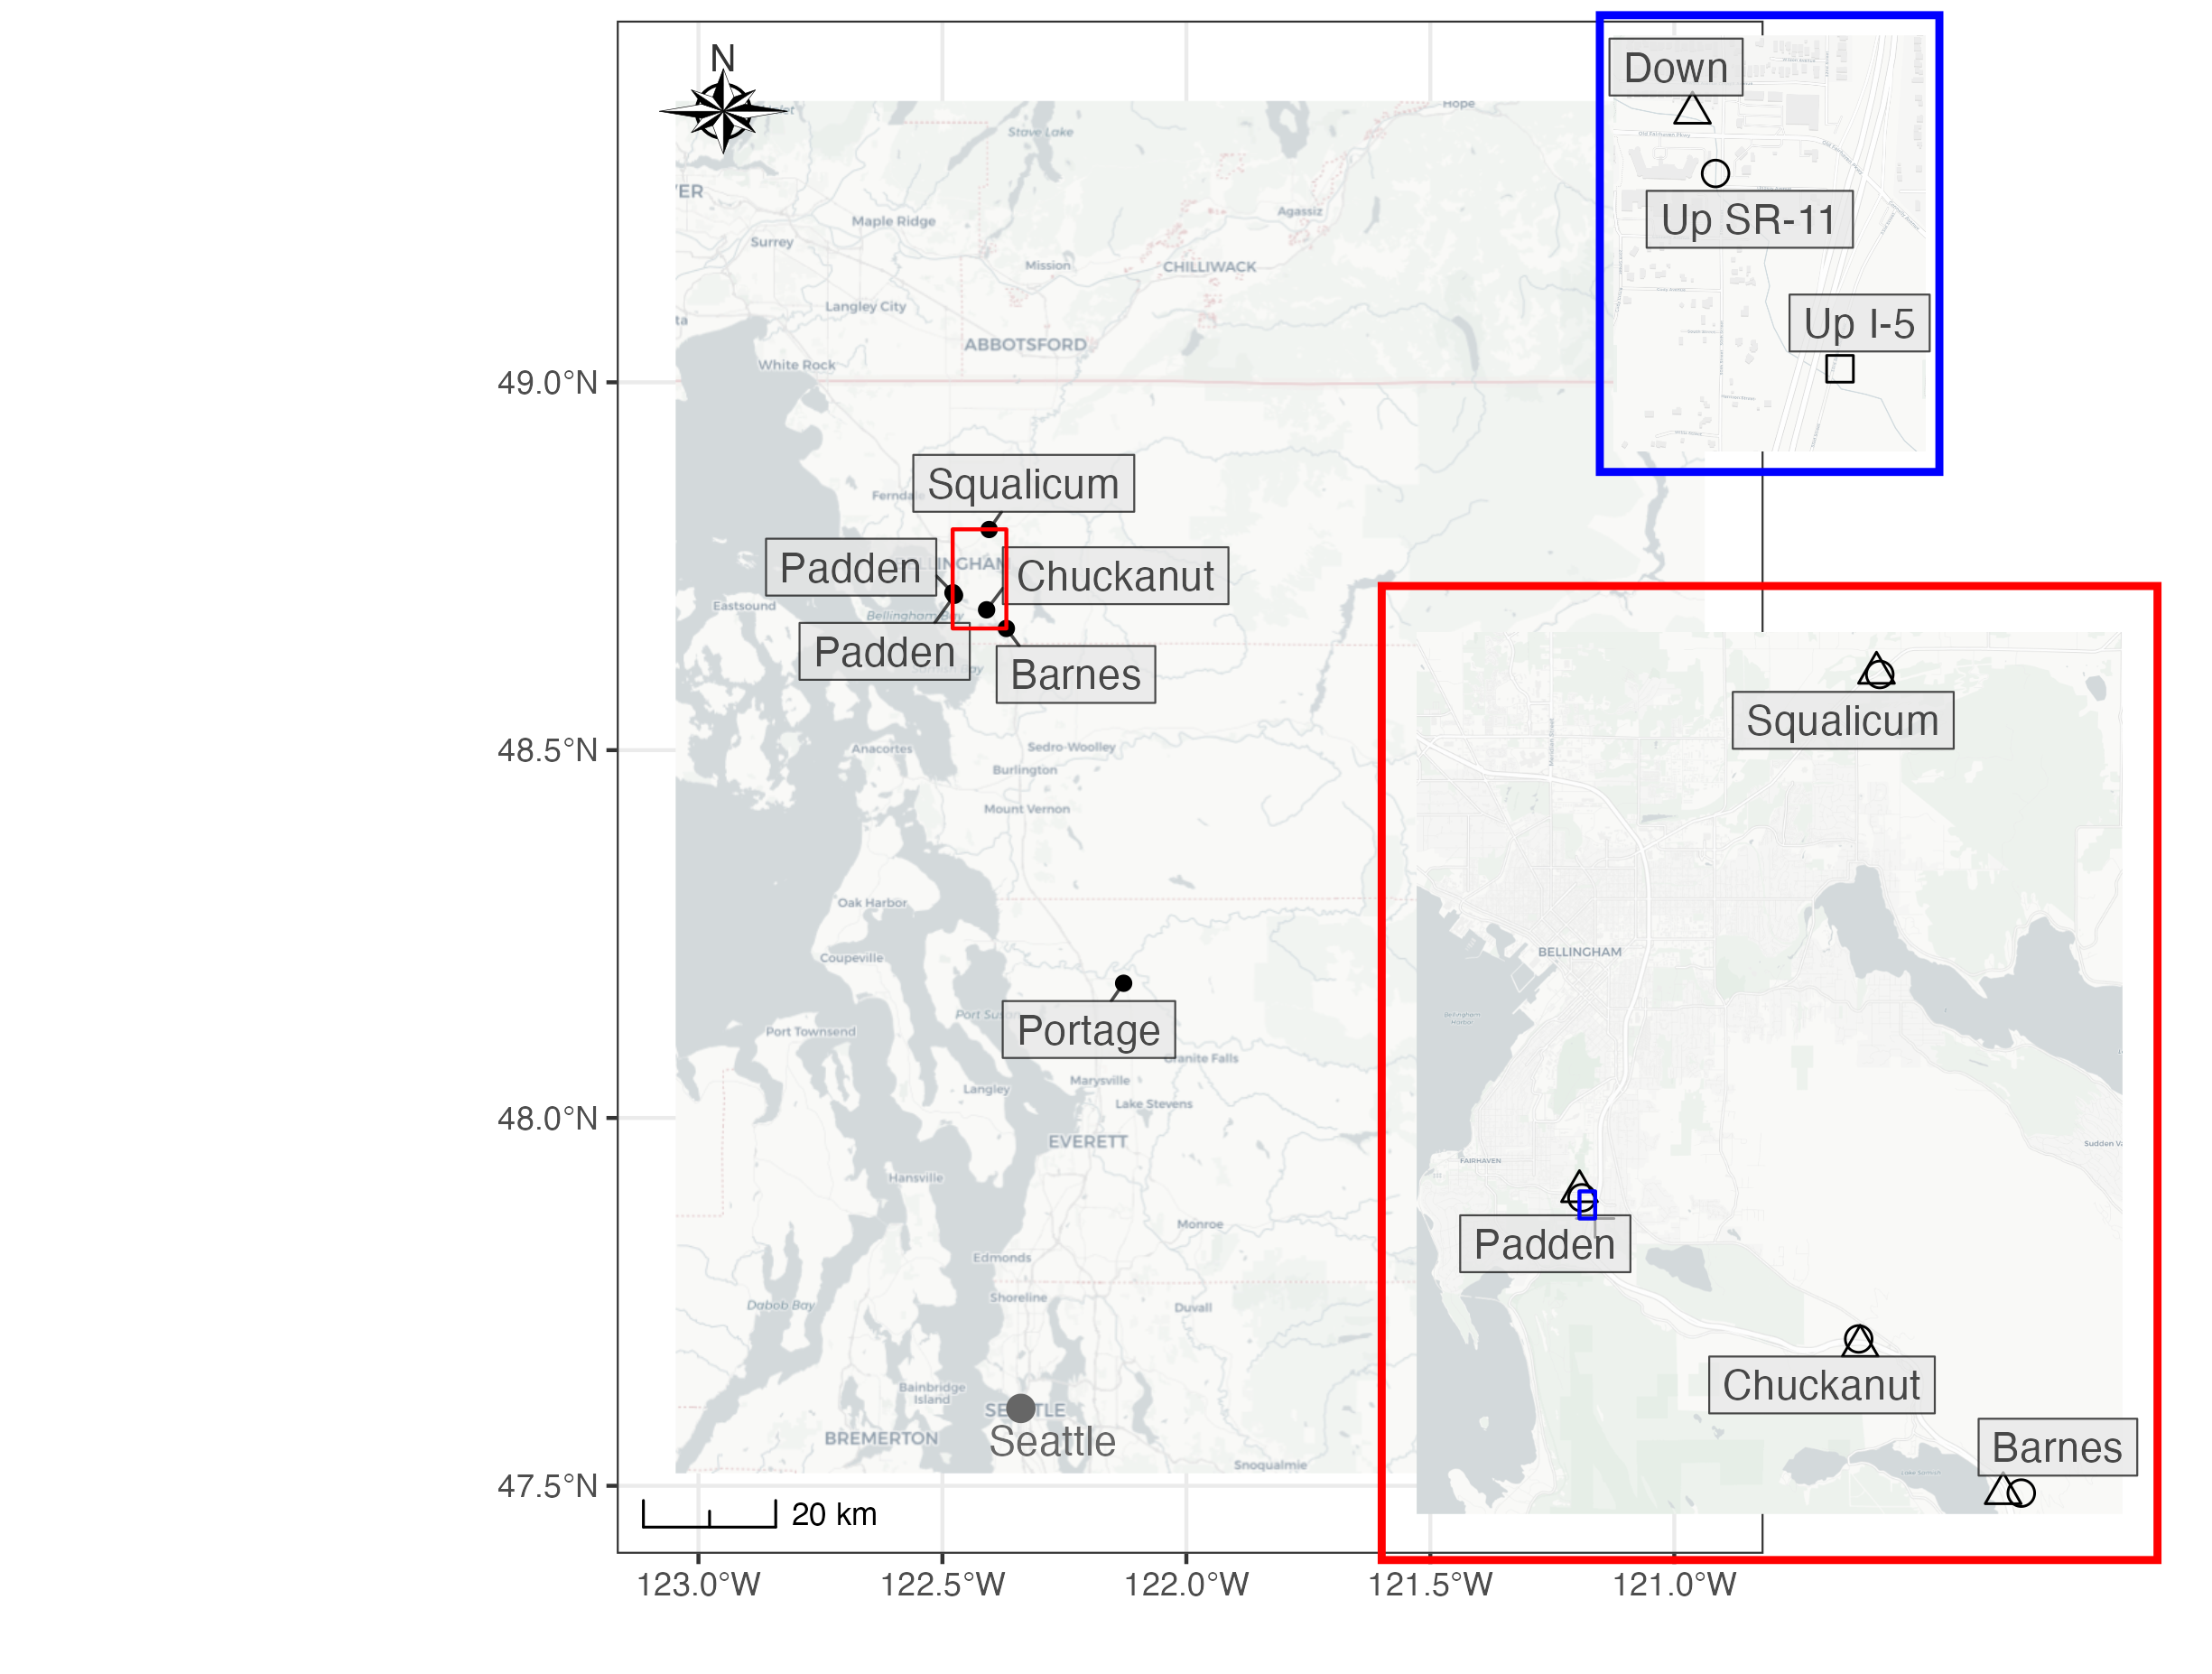
\includegraphics{../Output/Figures/SiteMap.png}
\caption{Map of sampling locations near Bellingham, Washington. In the
subset, open triangles designate the downstream sampling location and
open circles designate the upstream sampling location. Padden Creek is
the treatment creek where the culvert was replaced.\label{fig:map}}
\end{figure}

The intervention (i.e., culvert replacement) in Padden Creek occurred
over about two months and included the ``de-watering'' of the creek,
removal of the existing culvert, installation of the new culvert, and
then the ``re-watering'' of the creek from late August 2021 to early
October 2021 (Supplemental Text 1; Supplemental Figure 3). We were then
able to quantify the effect of the culvert replacement itself --
controlling for temporal trends, background environmental variability,
and sampling variability -- using a Bayesian time-series model to
jointly model salmon eDNA abundances across creeks, time points,
sampling stations, and species.

Because salmonids are the primary species of management concern in these
creeks, we focus the present analysis on the four salmonid species most
common in our data: cutthroat trout (\emph{Oncorhynchus clarkii)}, coho
salmon (\emph{O. kisutch}), rainbow/steelhead trout (\emph{O. mykiss}),
and sockeye/kokanee salmon (\emph{O. nerka}). Not all four salmonids are
expected to be found in all five of the creeks sampled. As documented by
WA Department of Fish and Wildlife SalmonScape
(\url{http://apps.wdfw.wa.gov/salmonscape/map.html}), all creeks contain
cutthroat trout, steelhead trout, and coho salmon. Barnes Creek is the
only creek documented to have kokanee salmon (freshwater sub-type of
sockeye salmon). However, local spawner surveys conducted by the City of
Bellingham from 2015-2020 in Padden Creek documented kokanee salmon, as
well as the other three species and importantly, several unknown species
of live and dead fish and redds (nests dug by fish in gravel to deposit
eggs) (City of Bellingham 2015). The four salmonid species in this study
have different life histories and behaviors that would impact when fish
(and therefore eDNA concentrations) occur in the creeks . Furthermore,
three of the four species in this study have both freshwater resident
and saltwater migrating behavior. For the fish exhibiting migratory
behavior , the run timings vary for each species in the study area (see
Discussion and Supplemental Figure 3). Therefore, our eDNA
concentrations might reflect contributions from both migrating and
non-migrating individuals at any given time point in the dataset.

\hypertarget{water-sampling}{%
\subsubsection{Water Sampling}\label{water-sampling}}

We collected water samples monthly between March 2021 and February 2022.
At each sampling station (N=2, upstream and downstream of a culvert) at
each creek (N=5) in each month (N=12), we collected three 2-liter water
samples, for a total of 360 water samples. Samples were collected using
Smith Root's eDNA Backpack (Thomas et al. 2018), a portable
pumping-and-filtering device set to filter at 1 L/min at 82.7 kPa (12
psi). In some months, less than 2 L of water was filtered due to
clogging (min = 1.02 L, mean = 1.97 L, median = 2.01 L; see Supplemental
Figure 4). Water samples were filtered using single-use inlet tubes
through 5\(\mu\)m self-preserving filters (Smith Root, Vancouver, WA),
which were then dried and kept at room temperature until DNA extraction
within 1 month of collection (Thomas et al. 2019).

Over the course of the year of sampling, water discharge varied from
very low to no flow in summer months to high flow in winter months
(Figure \ref{fig:flow_gauges}). Thus, we need to account for the large
difference in water volume over the course of the year and thus dilution
by converting eDNA concentration {[}copies/\(\mu\)L{]} to an eDNA mass
flow rate {[}copies/s{]} by multiplying eDNA concentrations by discharge
{[}L/s{]} (Tillotson et al. 2018, Thalinger et al. 2019). Flow gauges
maintained by the United States Geological Survey (USGS) were used for
Padden Creek (USGS Gage 12201905), Chuckanut Creek (USGS Gage 12201700),
and Squalicum Creek (USGS Gage 12204010;
\url{https://maps.waterdata.usgs.gov/mapper/index.html}; U. S.
Geological Survey (1994); Supplemental Figure 1). During the year of
sampling, the flow gauges at Chuckanut Creek and Squalicum Creek became
inoperable after a major flooding event. To find discharge rates for
Chuckanut and Squalicum Creeks, five years of historical data
(2015-2020) were used to generate a monthly averaged correction factor
based on Padden Creek. For the year of sampling (2021-2022), the
discharge rates used at Chuckanut and Squalicum Creeks were estimated
based on the correction factor from Padden Creek (Supplemental Figure
2). No discharge data was available for Portage Creek or Barnes Creek.
Based on field sampling conditions, the discharge from Padden Creek was
used as a proxy for both Portage and Barnes as they are in similarly
sized watershed areas and land-cover characteristics. Though in the year
of sampling, the discharge in Padden Creek ranged from no metered flow
to 23 m\textsuperscript{3}/s, the discharge on the dates of sampling
only reached a maximum of 1.3 m\textsuperscript{3}/s.

\begin{figure}
\centering
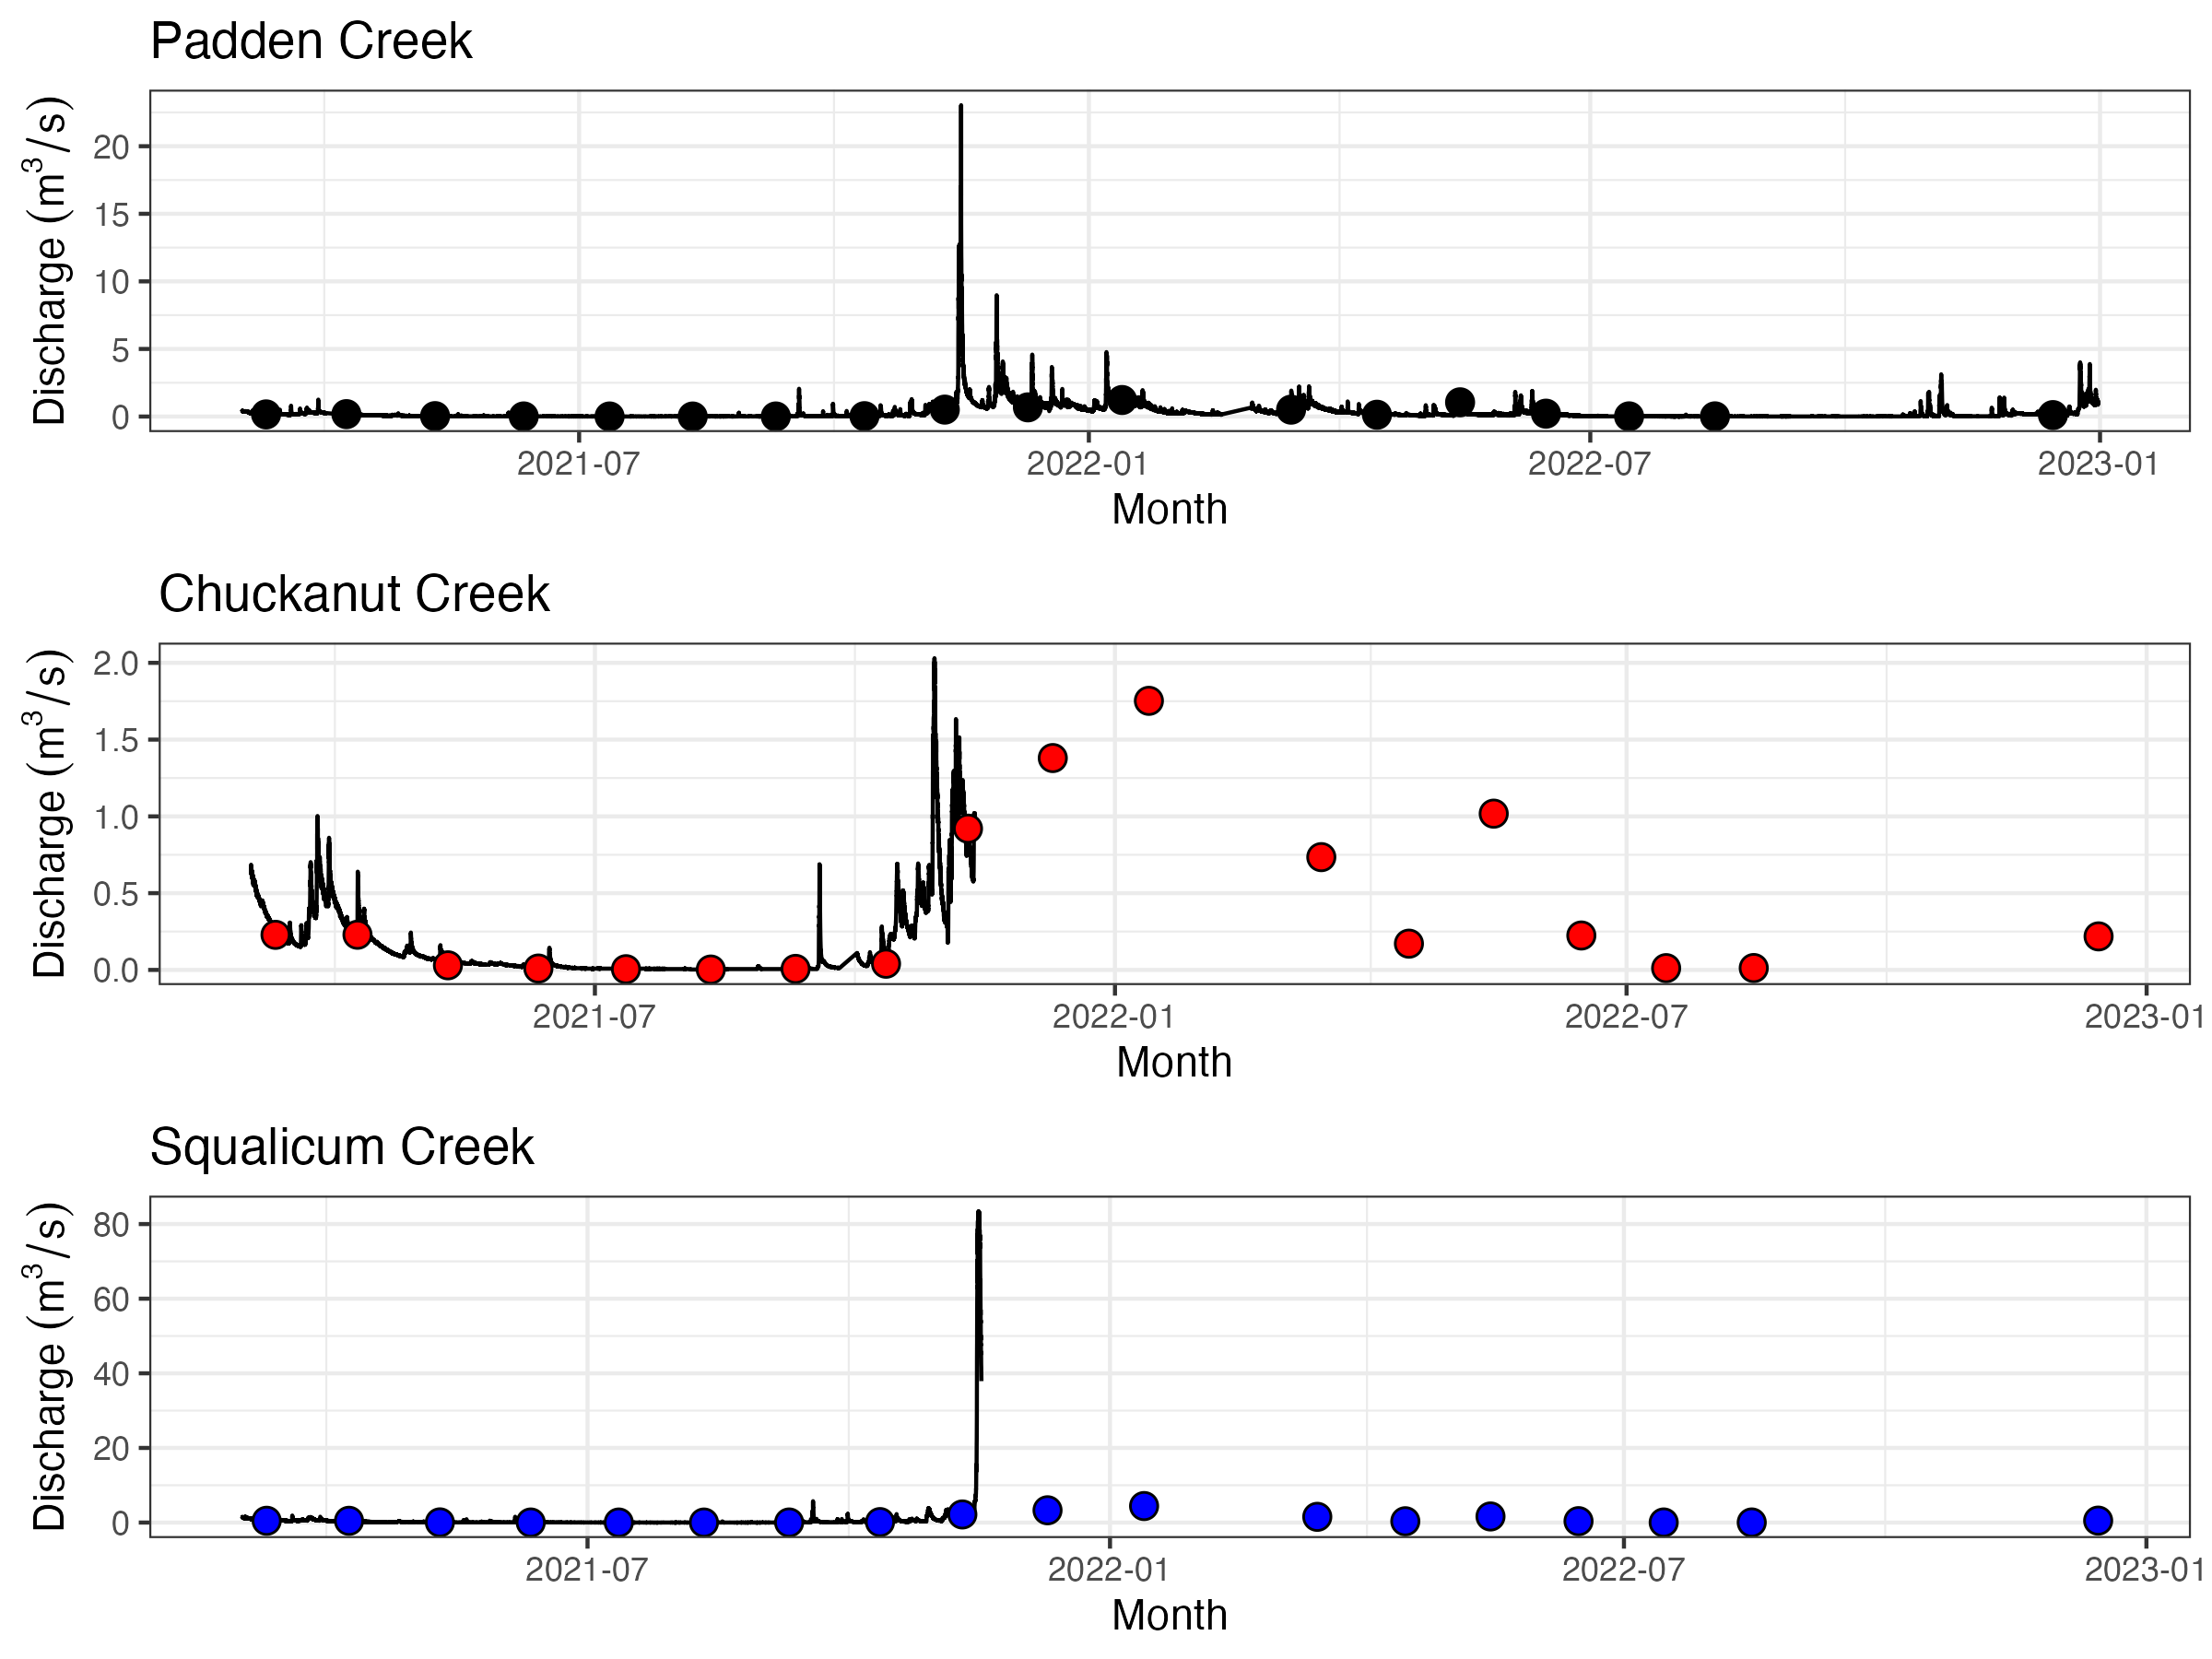
\includegraphics{../Output/Figures/flow_gauges.png}
\caption{Discharge (m\textsuperscript{3}/s) in Padden (USGS Gage
12201905), Chuckanut (USGS Gage 12201700), and Squalicum (USGS Gage
12204010) Creeks over the course of sampling. Open circles show the days
when sampling occurred. Gauges at Chuckanut and Squalicum Creek went
offline in November 2021 after a major storm event. Portage Creek and
Barnes Creek did not have stream gauges.\label{fig:flows}}
\end{figure}

Additionally, in the creek of interest, Padden Creek, rainbow trout
(\emph{O. mykiss}) were stocked in Lake Padden, approximately 1.5 km
upstream of the sampling sites. Occasionally, cutthroat trout (\emph{O.
clarkii}) and kokanee salmon (\emph{O. nerka}) have been stocked in the
past as well. During the course of the study, a total of 10,000 rainbow
trout were stocked in April and May 2021 and 30,000 kokanee salmon were
stocked in May 2021 (Supplemental Figure 3). Despite the stocking of
30,000 kokanee salmon in May in Lake Padden, \emph{O. nerka} was only
detected by metabarcoding in March 2021, August 2021, and then November
2021 through February 2022 (see Results below). Importantly, this
suggests that Lake Padden is far enough upstream that the eDNA signal at
the sampling sites by the culvert is not a result of stocking the lake
1.5 km upstream (see Discussion for more information).

\hypertarget{dna-extraction-amplification-sequencing}{%
\subsubsection{DNA Extraction, Amplification,
Sequencing}\label{dna-extraction-amplification-sequencing}}

All molecular work prior to sequencing was performed at the University
of Washington. Details of the molecular work can be found in
Supplemental Text 1. Briefly, DNA was extracted off filters using a
Qiashredder column (Qiagen, USA) and the DNeasy Blood and Tissue Kit
(Qiagen, USA) with an overnight incubation (Supplemental Text 1, Thomas
et al. (2019)). Extracts were stored at -20\degree C until PCR
amplification within 2 months of extraction.

For the metabarcoding approach, we targeted a \textasciitilde186 bp
hypervariable region of the mitochondrial DNA 12S rRNA gene for PCR
amplification (MiFish; Miya et al.~2015), but using modified primer
sequences as given in Praebel and Wangensteen (unpublished; via personal
communication). The primer sequences, final reaction recipe, and cycling
conditions can be found in Supplemental Text 1. Each month of samples
was amplified on a single plate with the addition of a no template
control (NTC; molecular grade water in lieu of template) and a positive
control (genomic DNA from kangaroo). PCR products were visualized,
size-selected, and diluted iteratively if inhibited. After cleaning, a
second PCR amplification added unique indices to each sample using
Nextera indices (Illumina, USA) to allow pooling multiple samples onto
the same sequencing run (See Supplemental Text 1 for details). Indexed
PCR products were also size-selected and visualized before pooling for
sequencing. Samples were randomized in 3-month blocks and each block
split across 3 sequencing runs, for a total of 12 sequencing runs. The
loading concentration of each library was 4-8 pM and 5-20\% PhiX was
included depending on the composition of the run. Sequencing was
conducted using an Illumina Miseq with v3 2x300 chemistry at the NOAA
Northwest Fisheries Science Center and the University of Washington's
Northwest Genomics Center.

Here, we used mock communities to determine the species-specific
amplification efficiencies for each salmonid in the study. Briefly, we
constructed five communities with known proportions of starting DNA from
different species (total DNA as measured by Qubit). The communities
ranged from having a total of 12 to 20 species, but six salmonid species
were included in all five mock communities to have more information on
the amplification efficiencies of salmonids (Supplemental Table 3). We
sequenced these communities using the same metabarcoding primers and
thermocycling conditions above and then determined the species-specific
amplification rates given the discrepancy between the known starting
proportion and the proportion of reads after sequencing. The mock
community data were then used to correct the sequencing reads from the
environmental samples to estimate the starting DNA proportions of each
species in environmental samples, which is the metric of interest
(Figure 3, green boxes). This is the first application of the model to
correct eDNA data from water samples with mock community data as
described in Shelton et al. (2022) (see Supplemental Text 2 for more
information).

\hypertarget{bioinformatics}{%
\subsubsection{Bioinformatics}\label{bioinformatics}}

After sequencing, bioinformatic analyses were conducted in R (R Core
Team 2017). A more detailed description of the bioinformatics pipeline
is included in the supplement (Supplemental Text 1). Briefly, primer
sequences were removed using \emph{Cutadapt} (Version 1.18) (Martin
2011) before \emph{dada2} (Callahan et al. 2016) trimmed, filtered,
merged paired end reads, and generated amplicon sequence variants
(ASVs). Taxonomic assignment was conducted via the \emph{insect} package
(Wilkinson et al. 2018) using a tree generated by the developers for the
MiFish primers that was last updated in November 2018. Only species
level assignments from \emph{insect} were retained and ASVs not
annotated or not annotated to species level were then checked against
the NCBI nucleotide database using BLAST+ (Camacho et al. 2009). Query
sequences that matched a single species at \textgreater95\% identity
were retained.

\hypertarget{quantitative-pcr-and-inhibition-testing}{%
\subsubsection{Quantitative PCR and Inhibition
Testing}\label{quantitative-pcr-and-inhibition-testing}}

We quantified cutthroat trout (\emph{O. clarkii}) DNA in each sample,
targeting a 114 bp fragment of the cytochrome b gene with a qPCR assay
(Duda et al. 2021). The primer/probe sequences, final recipe, and
thermocycling conditions can be found in Supplemental Text 1. Each DNA
sample was run in triplicate and was checked for inhibition using the
EXO-IPC assay. The majority of environmental samples (65\%) were
inhibited and accordingly diluted for analysis. In 75\% of inhibited
samples, a 1:10 dilution remedied the inhibition, but some samples
required dilution by a factor of up to 1000 (Supplemental Figure 5).
Each plate included a 8-point standard curve created using synthetic DNA
(gBlocks) ranging from 1 to 100,000 copies/\(\mu\)L and six no template
controls (NTCs) were included on each plate with molecular grade water
instead of template. Plates were re-run if efficiency as determined by
the standard curve was outside of the range of 90-110\%. All qPCRs were
conducted on an Applied Biosystems StepOnePlus thermocycler.

All qPCR data was processed in R using Stan (Stan Development Team
2022), relating environmental samples to the standard curve via a linear
model (Figure \ref{fig:conceptualfig}, blue boxes). We amended the
standard linear regression model to more realistically capture the
behavior of qPCR observations, accommodating non-detections as a
function of underlying DNA concentration, and letting the standard
deviation vary with the mean (lower-concentration samples had more
uncertainty). See McCall et al. (2014) and Shelton et al. (2019) for
similar models; see Supplemental Text 2 for full statistical details.
Subsequent analysis corrected for sample-specific dilution if found
inhibited and corrected for any variation in water-volume filtered
during sample collection.

\hypertarget{quantitative-metabarcoding}{%
\subsubsection{Quantitative
Metabarcoding}\label{quantitative-metabarcoding}}

The intercalibration of the mock community samples demonstrated the rank
order of amplification efficiencies for salmonids (Supplemental Figures
14 and 15). Cutthroat trout (\emph{O. clarkii}) and sockeye/kokanee
salmon (\emph{O. nerka}) had similar amplification efficiencies, both of
which were higher than rainbow/steelhead trout (\emph{O. mykiss}) and
coho salmon (\emph{O. kisutch}), which had the lowest amplification
efficiency. Calibrated metabarcoding analysis yielded quantitative
estimates of the proportions of species' DNA in environmental samples
prior to PCR. We then converted these proportions into absolute
abundances by expansion, using the qPCR results for our reference
species, \emph{O. clarkii}. We estimated the total amplifiable salmonid
DNA in environmental sample \(i\) as
\(\text{C}_{\text{amplifiable}_{i}} = \frac{\text{C}_{\text{qPCR reference}_{i}}}{\text{Proportion}_{\text{reference}_{i}}}\),
where C has units of {[}DNA copies/uL{]} and then expanded species'
proportions into absolute concentrations by multiplying these
sample-specific total concentrations by individual species' proportions,
such that for species \(j\) in sample \(i\),
\(\text{C}_{i,j} = \text{C}_{\text{amplifiable}_{i}} * \text{Proportion}_{i,j}\).
Here, we combine the modeled output of the qPCR model for cutthroat
trout (Figure \ref{fig:conceptualfig} dashed blue box) and modeled
proportions of salmonid DNA from metabarcoding (Figure
\ref{fig:conceptualfig} dashed green box). Though in the future this
could be used as a joint model, here the precision of our modeled
estimates were very high such that we used the mean of the posterior
estimates from each model to move forward as input to the time series
model (Figure \ref{fig:conceptualfig} dashed purple box; see
Supplemental Text 2 for more details). Finally, due to the range of
water discharge over the course of the year, we converted from DNA
concentration {[}copies/L{]} to a mass flow rate {[}copies/s{]} after
multiplying by the discharge of each creek {[}m\textsuperscript{3}/s{]}
(Figure \ref{fig:conceptualfig}, solid purple boxes).

\begin{figure}
\centering
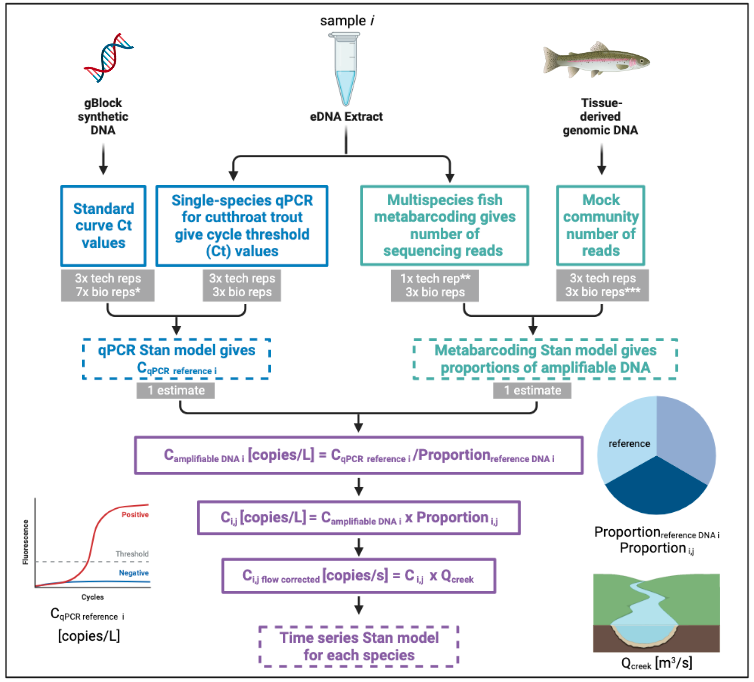
\includegraphics{../Output/Figures/conceptual_figure.png}
\caption{Conceptual figure of different datasets and models used for
analyses. * indicates that here, biological replicates are different
dilutions of the synthetic gBlock. ** indicates that for most samples,
only one technical replicate was sequenced but for one sample per
sampling month, three techincal replicates were sequenced to check for
consistency across replicates. *** indicates that here, the three
biological replicates indicate three different mock communities with
varying species compositions, but all containing the four salmonids of
interest.\label{fig:conceptualfig}}
\end{figure}

\hypertarget{estimating-the-effects-of-culvert-replacement-and-of-culverts-themselves}{%
\subsubsection{Estimating the Effects of Culvert Replacement and of
Culverts
Themselves}\label{estimating-the-effects-of-culvert-replacement-and-of-culverts-themselves}}

We sampled four control creeks as context against which to compare the
observations in Padden Creek, our treatment creek where the culvert was
being replaced. Recognizing that these observations are autocorrelated
in time, we use an AR(1) autocorrelation model, implemented in Stan via
R, to capture the observed temporal trends.

We observe the log-DNA concentration, \(Y\), for a given species in a
given sample as a random variable drawn from a normal distribution with
mean \(\mu\) and observation variance \(\sigma^2\). For each species
\(j\), the expected log-DNA concentration \(\mu\) at time \(t\) in creek
\(i\) at station \(d\) is a linear function of the DNA concentration for
the same creek/station at \(t-1\).

\begin{align*}\label{eqn:ts}
Y_{i,j,t,d} &\sim \mathcal{N}(\mu_{i,j,t,d},\,\sigma^{2})\\
\mu_{i,j,t,d} &= \alpha_{i,j,t} + \epsilon_{i,j,t,d} + \eta_{i,j,t,d}\\
\epsilon_{i,j,t,d} &\sim \mathcal{N}(\beta_{j}\mu_{i,t-1,d},\, \phi^2)
\end{align*}

Intercept \(\alpha\) varies by time, creek, and species, capturing
creek-level deviations from the previous time-step. The autoregression
term \(\epsilon\) is itself a random variable drawn from a normal
distribution with expected value \(\beta_{j}\mu_{i,t-1,d}\) and process
variance \(\phi^2\), such that the species-specific slope term
\(\beta_{j}\) estimates the degree of autocorrelation in log-DNA
concentration between one time-step and the next. The model shares
information across creeks and time-points via \(\beta_{j}\).

Finally, \(\eta\) captures the difference in log-DNA concentration
between upstream and downstream stations within a creek; we set
\(\eta_{d = 1} = 0\) such that the value of \(\eta_{d = 2}\) explicitly
captures the effect of the culvert within a given creek at a given time.
The effect of construction in our focal Padden Creek, then, is the
change in \(\eta\) after construction versus prior to construction. We
fit this model in a Bayesian framework using moderately informative
priors on all parameters, and confirmed model convergence
(\(\hat{R} < 1.01\)) across 3 chains and 3500 model iterations. See
statistical supplement (Supplemental Text 2) for prior values,
diagnostics, and full model details.

\hypertarget{results}{%
\subsection{Results}\label{results}}

\hypertarget{metabarcoding-and-quantitative-pcr}{%
\subsubsection{Metabarcoding and Quantitative
PCR}\label{metabarcoding-and-quantitative-pcr}}

In total, sequencing runs generated \textasciitilde42 million reads
across all environmental samples (12 months x 2 stations x 5 creeks x 3
biological replicates = 360 filters) and 27 mock community samples (3
communities x 9 replicates {[}6 even, 3 skewed proportions{]}) for
calibration (see below). After quality-filtering and merging all runs,
\textasciitilde33 million reads remained from \textasciitilde21,000
amplicon sequence variants (ASVs) in the environmental samples, of which
\textasciitilde81\% of reads were annotated to species level (per
sample: mean = 78\%, median = 88\%, min = 0\%, max = 99.99\% of reads
annotated). We only focus on the metabarcoding data from four salmonids
for the remainder of this paper. The four salmonids represent
\textasciitilde68\% of the annotated reads found in environmental
samples.

In the mock community samples, 98.7\% of the \textasciitilde5 million
reads after quality filtering were annotated to species level.
Importantly, the target salmonid ASVs in the mock communities were found
in environmental samples, unambiguously linking the taxa in calibration
samples with those in environmental samples. The most common salmonid
species found in the environmental samples was cutthroat trout (\emph{O.
clarkii}), which was found in \textasciitilde90\% of samples, followed
by coho salmon (\emph{O. kisutch}) found in \textasciitilde60\% of
samples, then rainbow/steelhead trout (\emph{O. mykiss}) found in
\textasciitilde40\% of samples, and finally sockeye/kokanee salmon
(\emph{O. nerka}) found in \textasciitilde5\% of samples. Not only was
cutthroat trout (\emph{O. clarkii}) found in the majority of
environmental samples, but also \textasciitilde63\% of samples across
all times, creeks, and stations had at least 50\% of reads assigned to
cutthroat trout.

After calibrating metabarcoding data using mock communities (See
Supplemental Texts 1 and 2), we estimated the salmonid composition
across time points, creeks, and stations (Figure \ref{fig:qm}). The
culvert in one control creek (Barnes) appeared to be nearly a total
barrier to salmonid passage, with salmonid eDNA detected upstream of the
culvert at only three time points, in contrast to being detected at
every time point in the downstream station of the same creek. The other
four creeks had no such pattern associated with the culverts, suggesting
that fish passage may have been possible through the culverts, or that
there were resident populations upstream of the culverts.

\begin{figure}
\centering
\includegraphics{../Output/Figures/proportions_after_qm.png}
\caption{Compositions of salmonid DNA as determined by metabarcoding
after correction for amplification bias. Note that no sampling occurred
in September 2021 at Squalicum Creek because the creek was dry. The
empty bars in the Barnes upstream sites indicate that no salmonid DNA
was found at those time points. The vertical dashed line in Padden Creek
indicates the time period in which the culvert was
replaced.\label{fig:qm}}
\end{figure}

All environmental samples were quantified for absolute concentrations of
cutthroat trout DNA across 30 qPCR plates, resulting in 280 samples
(\textasciitilde80\%) with a positive detection in at least 1 of 3
technical replicates. The modeled output of cutthroat trout DNA
concentrations, ranged from 10 copies/L to 1.4 x 10\textsuperscript{6}
copies/L, with a mean value of \textasciitilde58,000 copies/L (Figure
\ref{fig:qpcr}).

\begin{figure}
\centering
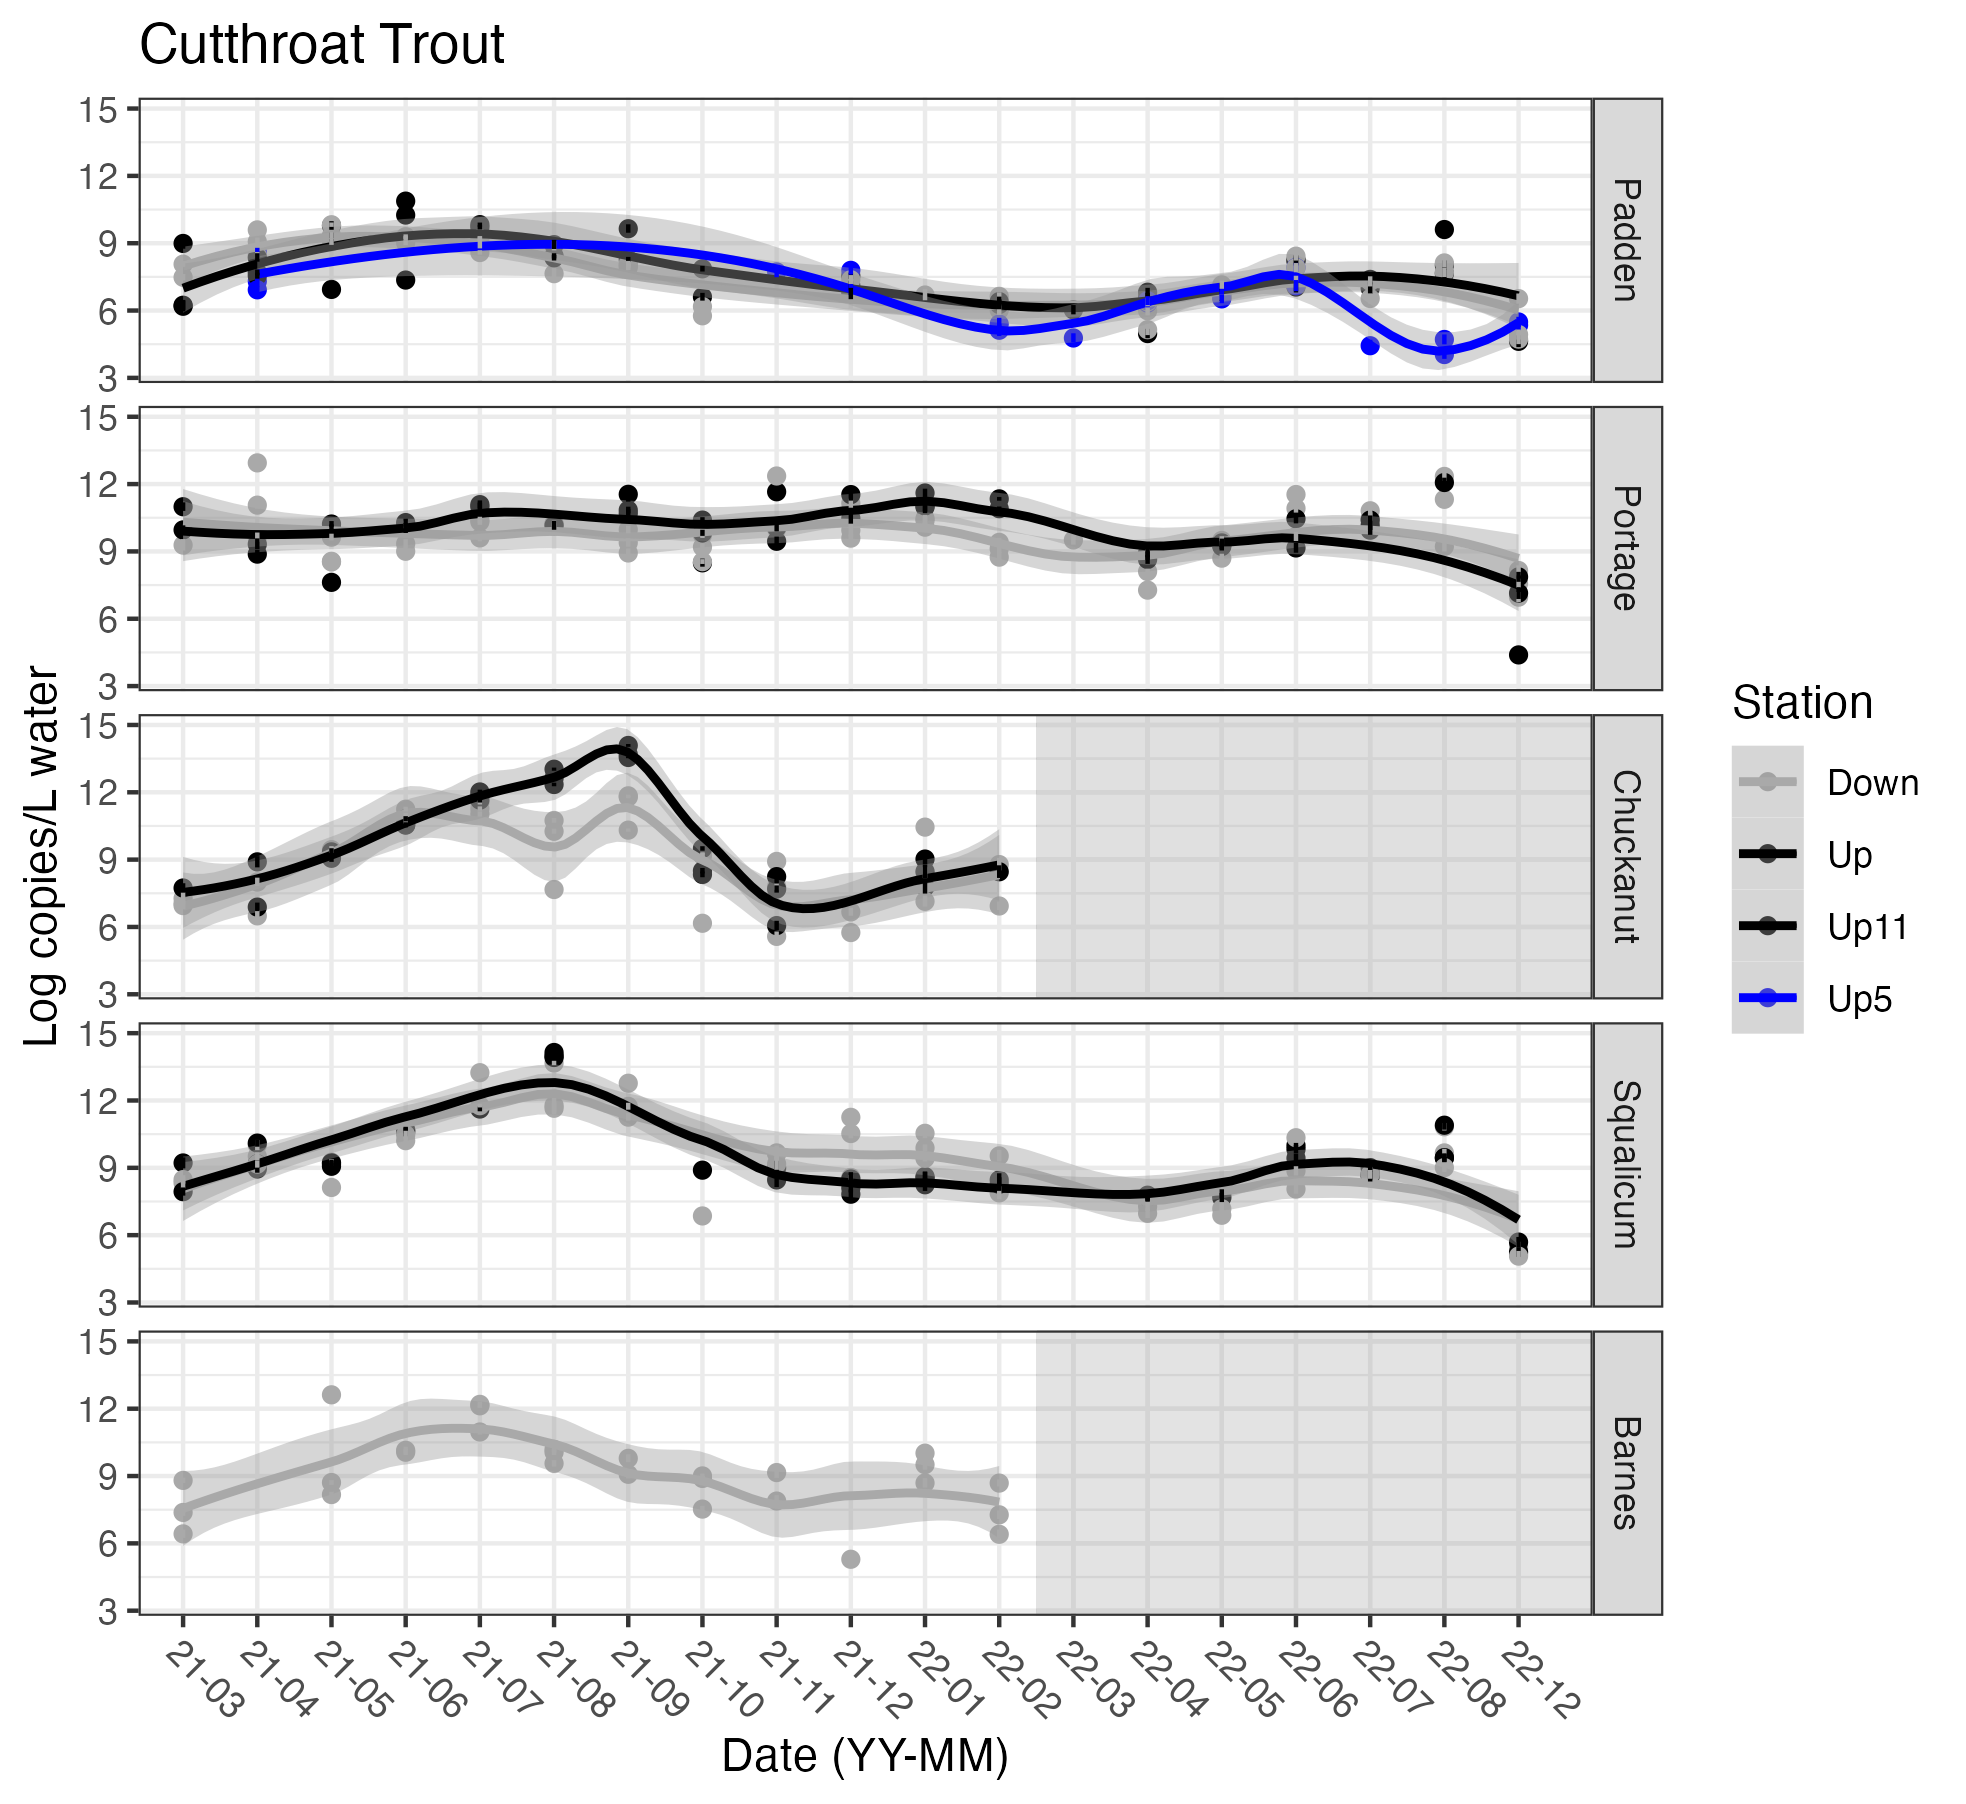
\includegraphics{../Output/Figures/modeled_cut_qpcr_updown-line.png}
\caption{Absolute concentration (log copies/L of water) of cutthroat
trout (\emph{O. clarkii}) as measured by qPCR before flow
correction.\label{fig:qpcr}}
\end{figure}

We combined compositional information from metabarcoding with absolute
concentrations for our reference species, cutthroat trout (\emph{O.
clarkii}), from the qPCR to estimate the total concentration of DNA for
each species (See Supplemental Text 2). The joint time-series model
shared information across stations and creeks; consequently, data from
one of the control creeks (Barnes) could not be included because of the
nearly total absence of salmonids upstream of its culvert. However, data
from the remaining creeks characterized trends in the other four target
species well and could be modeled appropriately (Figure \ref{fig:ts}).

\begin{figure}
\centering
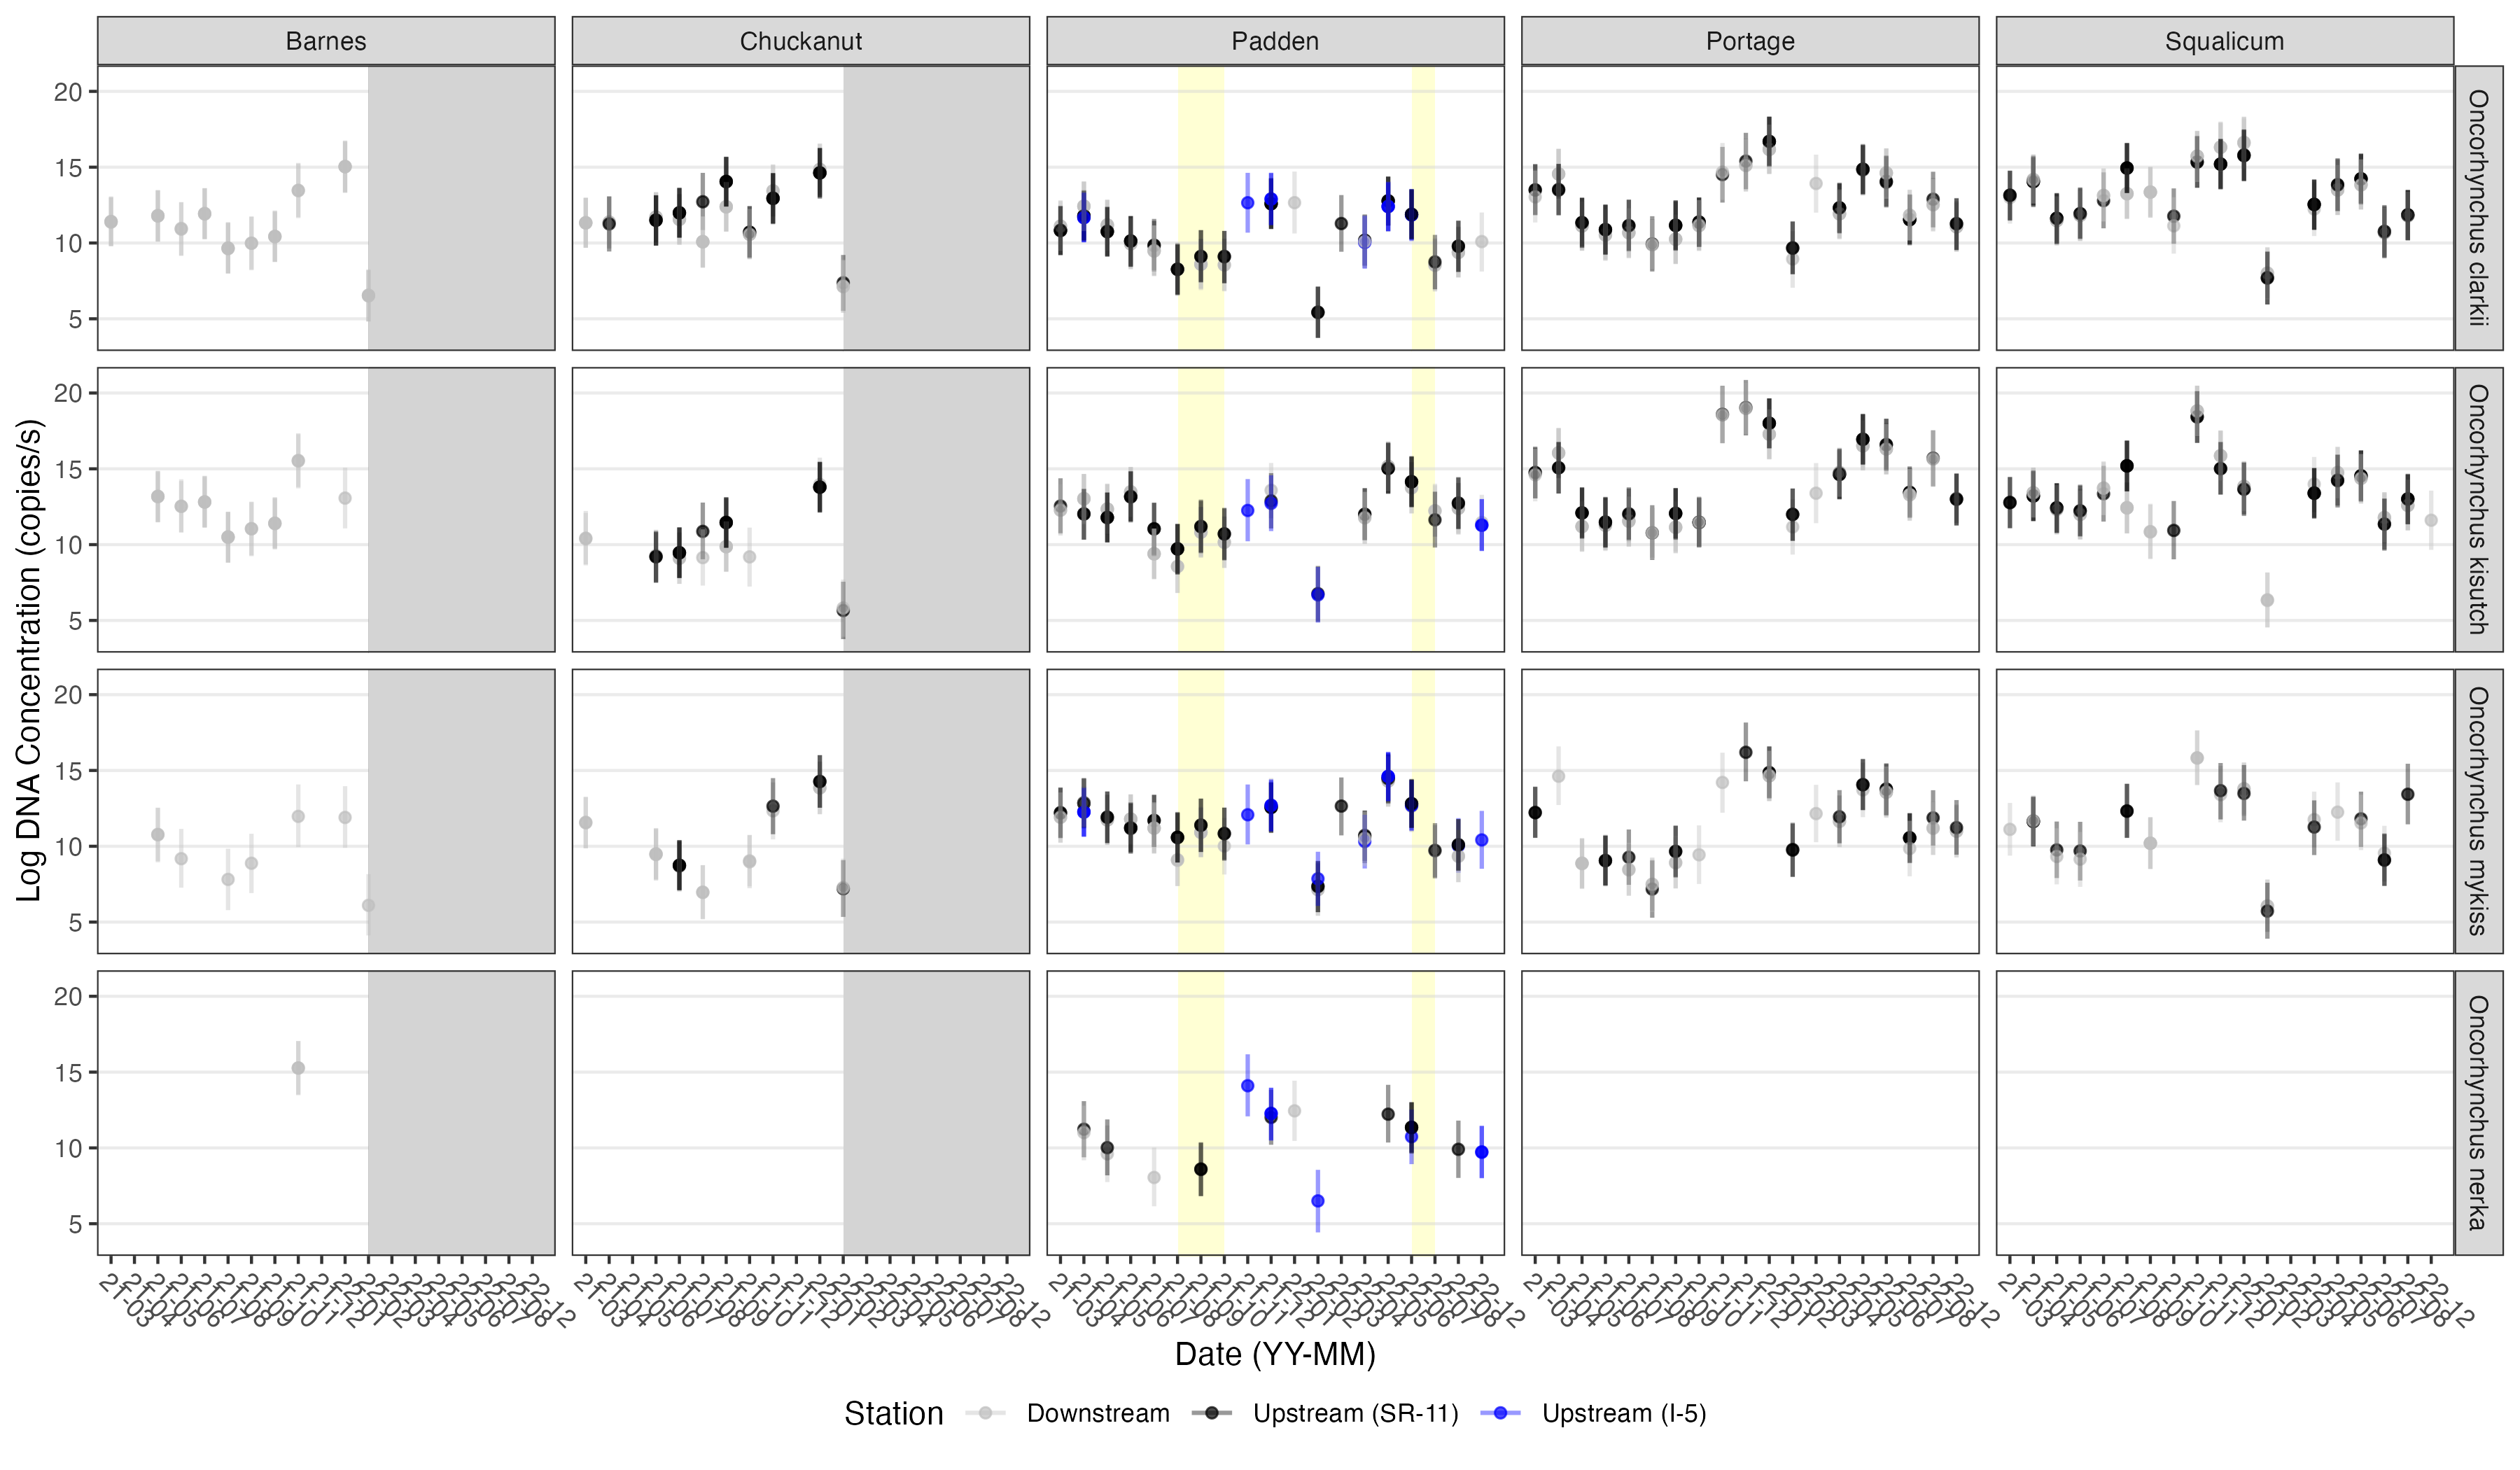
\includegraphics{../Output/Figures/multispeciesTrends_flowcorrected.png}
\caption{Trends across creeks and across time for each of four salmonid
species as estimated by eDNA analysis. Points represent posterior means
for the time-series model and error bars represent the 75\% posterior
confidence interval. Colors indicate station upstream or downstream of
an under-road culvert. Grey shading indicates the time period in which
the culvert in the treatment creek (Padden Creek) was
replaced.\label{fig:ts}}
\end{figure}

\hypertarget{effects-of-culverts}{%
\subsubsection{Effects of Culverts}\label{effects-of-culverts}}

Before considering the effect of construction, the difference in
abundance trends between upstream and downstream stations (Figure
\ref{fig:ts}) demonstrates that the culverts themselves have some
effect, but not a large effect on the salmonid species surveyed.
Therefore, these four creeks (which range in how they are classified in
fish passability) do not seem to be blocking salmonid passage. A notable
exception was Barnes Creek, which was not included in the time series
model, as the culvert was so clearly a barrier as most time points had
no salmonid DNA upstream and therefore models including Barnes do not
converge as a result of the large fraction of sampling points with no
observations of salmonids. (Figure \ref{fig:qm}).

Summarizing over all species and the four creeks used in the time series
model, the culvert effect was minimal (Figure \ref{fig:culverts}); the
difference between upstream and downstream concentrations (normalized by
upstream concentration) was on average only about 3\%, indicating
slightly higher concentrations upstream across creeks and species.
Across species and times but within each creek, Chuckanut had the
largest difference, followed by Portage, Padden, and Squalicum. In terms
of species across time and creeks, rainbow trout (\emph{O. mykiss}) saw
the largest difference, followed by coho (\emph{O. kisutch}), cutthroat
(\emph{O. clarkii}), and sockeye (\emph{O. nerka}). Late summer / fall
(August 2021 - October 2021) seemed to have the largest difference
between upstream and downstream, which corresponds with when flows were
at a minimum (i.e., August and September had lowest averge flows across
creeks) and the connectivity between upstream and downstream was low
(Figure \ref{fig:culverts}). Individual species' patterns were similar,
indicating that there is not a species-specific effect where culverts
block the passage of some salmon but not others (Supplemental Figure
17). Across all species and time points, Squalicum Creek had the lowest
mean percent difference in upstream and downstream salmonid DNA
concentrations.

\begin{figure}
\centering
\includegraphics{../Output/Figures/culvert_effect_flowcorrected.png}
\caption{The effect of culvert on salmonid abundance summed across all
species and creeks by time. The y-axis shows the difference between
upstream and downstream concentrations, normalized by upstream
concentration. The box boundaries correspond to the 25th and 75th
percentiles; the whiskers correspond to 1.5 times the interquartile
range. Here, negative values imply that eDNA concentrations are higher
downstream than upstream. Samples with very low eDNA mass flow rates
(\textless{} 150 copies/s) were removed before plotting to remove
extreme proportional values due to large
denominators.\label{fig:culverts}}
\end{figure}

\hypertarget{effects-of-culvert-replacement}{%
\subsubsection{Effects of Culvert
Replacement}\label{effects-of-culvert-replacement}}

By comparing the difference in upstream and downstream concentrations
before and after construction in Padden Creek, we can assess how large
of an impact the replacement had on salmonid species (Supplemental
Figure 3). The effects of the culvert replacement operation appeared to
have been transient and fairly minor for the four salmonid species
surveyed. After the beginning of construction in September 2021 through
the end of sampling in February 2022, we saw very minor fluctuations in
the difference between upstream and downstream salmonid DNA
concentrations, and did not see an increase in this difference due to
the culvert removal (Figure \ref{fig:construction}, grey shading vs.~no
shading). The mean percent difference across all species prior to
construction was 2.4\% compared to 1.5\% during and post-construction
(Supplemental Table 2).

\begin{figure}
\centering
\includegraphics{../Output/Figures/construction_legend.png}
\caption{Effect of Construction on Salmonid DNA Concentrations in Padden
Creek. Error bars show 75\% confidence intervals of the normalized
difference between upstream and downstream DNA concentrations. Grey
shading shows when construction started through the end of sampling.
Construction ended in early October 2022. Sockeye/kokanee salmon
(\emph{O. nerka}) was only found in Padden Creek so other creeks are not
shown. Samples with very low eDNA mass flow rates (\textless{} 150
copies/s) were removed before plotting to remove extreme proportional
values due to large denomenators.\label{fig:construction}}
\end{figure}

\hypertarget{discussion}{%
\subsection{Discussion}\label{discussion}}

\hypertarget{environmental-dna-can-provide-quantitative-measurements-of-environmental-impacts}{%
\subsubsection{Environmental DNA can provide quantitative measurements
of environmental
impacts}\label{environmental-dna-can-provide-quantitative-measurements-of-environmental-impacts}}

Here, we used both eDNA metabarcoding and a single species-specific qPCR
assay to rigorously quantify both the effect of culverts and the impact
of a culvert replacement on salmonids. We observed a clear seasonal
pattern in the DNA concentrations of four salmonid species detected in
the study. The sampling design and the time series model leveraged
shared information across creeks to integrate the change in eDNA
concentrations due to time, whether a sample was collected below or
above a barrier (i.e., culvert), and whether or not there was
construction occurring. Thus, we could isolate the changes in eDNA
concentrations as a result of the intervention (i.e., construction)
while accounting for the variance due to time and station (i.e., season
and culvert).

A few other studies have used eDNA to measure environmental impacts in
rivers and streams. Duda et al. (2021) used 11 species-specific qPCR
assays to document the distribution of resident and migratory fish after
a large dam removal project (Elwha River near Port Angeles, Washington).
No eDNA sampling was conducted before the dam removal, but the study
provided a wealth of information about species returning after the dam
removal, providing a very important dataset to use eDNA to monitor
ecological changes due to human intervention. Similarly, Muha et al.
(2017) sampled three locations upstream and three locations downstream
before and after the removal of a weir that was thought to be a barrier
to salmonid migrations. The authors only sampled once before and twice
after the removal, spanning about a year, and used eDNA metabarcoding to
look at the presence/absence of species detected. They found that in
fact the before sample demonstrated that the weir was not preventing
fish passage (similar to the results found in this study) and
furthermore documented a slight increase in alpha diversity in the first
time point after the barrier removal and then a return to a similar
alpha diversity in the second time point after the removal (similar
results found in this study using eDNA concentrations rather than
diversity).

Importantly, our study demonstrates the value of combining a single qPCR
assay with metabarcoding data to generate quantitative estimates of eDNA
concentrations of many species without requiring n qPCR assays for n
species of interest. Here, we ultimately only quantified the impacts of
four species, but importantly, we did not know \emph{a priori} how many
species of interest there might be and we reduced our efforts two fold
by only conducting two assays (one species-specific qPCR and one
metabarcoding assay) as opposed to four assays (four species-specific
qPCR assays). This can also be particularly helpful for taxa that don't
have a previously published qPCR assay, but are detected using universal
metabarcoding assays. Metabarcoding data alone only gives compositional
data, which cannot be used in a time series to quantify environmental
impacts because there is no information about absolute eDNA
concentrations. However, by anchoring or grounding proportions using a
single qPCR assay, the proportional data can be turned into quantitative
data. The species for which to run the qPCR assay can be determined
after the metabarcoding is completed; the most commonly found species
with a robust qPCR assay should be used to glean the most information.

\hypertarget{fish-life-histories-and-expected-patterns}{%
\subsubsection{Fish life histories and expected
patterns}\label{fish-life-histories-and-expected-patterns}}

The four salmonid species in this study have different life histories
and behaviors that would impact when fish (and therefore eDNA
concentrations) occur in the creeks. For these four migratory salmonids,
the run timings vary for each species in the study area (Bellingham,
WA). Adult coastal cutthroat (\emph{O. clarkii}) are documented to run
throughout the entire year, whereas coho salmon (\emph{O. kisutch}) run
from September to December, sockeye salmon (\emph{O. nerka}) run from
October to December, and steelhead trout (\emph{O. mykiss}) run from
November to June. For migrating coho (\emph{O. kisutch}) and steelhead
trout (\emph{O. mykiss}), juveniles may be present in the creeks
year-round (Supplemental Figure 3). Using eDNA methods, it cannot be
determined if the DNA found is sourced from adult or juvenile animals.

Furthermore, three of the four species in this study have both
freshwater resident and saltwater migrating behavior. Cutthroat trout
(\emph{O. clarkii}) encompasses both non-migrating, resident trout in
the creeks and coastal run cutthroat that migrate into Padden Creek from
saltwater (Bellingham Bay). Similarly, \emph{O. nerka} includes both
anadromous sockeye salmon and freshwater resident kokanee salmon and
\emph{O. mykiss} includes both anadromous steelhead trout and
non-migrating rainbow trout. Using eDNA, we cannot distinguish between
the migrating and non-migrating subspecies of \emph{O. clarkii},
\emph{O. nerka}, and \emph{O. mykiss}. Therefore, our eDNA
concentrations might reflect contributions from both migrating and
non-migrating individuals at any given time point in the dataset.

Despite the mix of migrating and non-migrating populations and various
run timings, our metabarcoding data demonstrate that in Padden Creek,
there was a clear signal of sockeye/kokanee salmon (\emph{O. nerka})
both upstream and downstream only in November 2021 - February 2022 (and
only upstream in March 2021). This signal corresponds well with the
documented run timing of October to December. In contrast, cutthroat
trout (\emph{O. clarkii}) and coho salmon (\emph{O. kisutch}) were found
nearly year-round in Padden Creek. The persistent signal from \emph{O.
clarkii} could be explained by resident cutthroat trout. However,
\emph{O. kisutch} does not have a resident subspecies and the run timing
is only documented from September to December. This could potentially be
due to juveniles maturing and residing in the creeks for 1-2 years after
hatching while adults migrate into the creeks only during the run time
to spawn. Visual surveys are conducted rarely and even if they were
conducted, it might be difficult to identify juveniles to species level.
Though \emph{O. kisutch} eDNA was found year round, the highest
concentrations were found near the expected run timing as expected and
the life history of \emph{O. kisutch} includes rearing year-round in
freshwater. Finally, though the lowest concentrations on average,
rainbow/steelhead trout (\emph{O. mykiss}) was also found nearly
year-round in Padden Creek, which could be contributions from migrating
steelhead (November to June), juveniles maturing and migrating, or from
resident rainbow trout. Though the \emph{O. mykiss} signal is found
year-round, the highest concentrations do seem to correspond with the
steelhead run timing.

\hypertarget{decoupling-of-edna-from-fish-abundance}{%
\subsubsection{Decoupling of eDNA from fish
abundance}\label{decoupling-of-edna-from-fish-abundance}}

By capturing residual eDNA from water samples, we are measuring a
different signal than counting how many fish are in the creek at each
time of sampling. We should not expect the eDNA concentration for each
salmonid to directly correlate to the number of fish in the creek at the
time of sampling, especially as we often did not visually see any fish
when we took water samples. Shelton et al. (2019) provides a paired eDNA
sampling and seine netting analysis demonstrating that eDNA
concentrations provide a smoothed biological signal over space and time.
We acknowledge this smoothing effect and emphasize that in the context
of using eDNA for environmental impact assessments, it is preferable to
use a survey technique such as eDNA that integrates signal across a
larger spatial and temporal scale.

Many previous papers have commented on the ``ecology'' of eDNA and the
various processes that contribute to eDNA concentrations in
environmental samples (e.g., shedding rates, decay rates, transport)
(Barnes and Turner 2015). For example, higher concentrations of eDNA
could be the result of a greater number (or biomass) of fish present, or
increased shedding rates, or decreased decay. Many review papers
document the nuances of interpreting eDNA data and we recommend
reviewing them for a deeper understanding (see Andruszkiewicz Allan et
al. (2020) for a review on shedding and decay rates and Harrison et al.
(2019) for a review on transport). Certainly eDNA concentrations can
arise from different scenarios and future work should continue to
investigate how to tease apart the nuances of relating eDNA
concentrations to fish abundance.

In this study, to assess the impact of a culvert on fish passage, we
compare eDNA concentrations upstream and downstream at the same time
point in a given creek. The distance between the upstream and downstream
sampling was minimal (\textasciitilde60-300 m, average distance of
\textasciitilde150 m). Therefore, we assume that the small differences
in spatial and temporal scale between sampling locations is minimal such
that the impacts of these various processes will affect the downstream
and upstream concentrations equally.

For assessing the impact of construction, we needed to account for
differences within the same creek over time (i.e., before and after
construction). Because the sampling occurred over a whole year,
transport and persistence times may have varied. However, the time
series model uses information from the control creeks to understand
seasonal trends in eDNA concentrations without needing to link eDNA
concentrations to fish abundance. The impact of construction in Padden
Creek can be understood by comparing the measured eDNA concentration
during the time of construction to the expected eDNA concentration in
the absence of construction by using information shared from the four
other creeks that are not undergoing construction. However, we did
correct eDNA concentrations {[}mass/volume{]} by discharge
{[}volume/time{]} and use a mass flow rate {[}mass/time{]} for the time
series model (see below) given the wide range of discharge over the
course of the year.

\hypertarget{accounting-for-flow-with-edna-concentrations}{%
\subsubsection{Accounting for flow with eDNA
concentrations}\label{accounting-for-flow-with-edna-concentrations}}

Though eDNA can move downstream with water flow, here, we were measuring
if culverts were barriers to fish moving upstream, as we were focused on
the impact of culverts on migratory salmon. In our case, we were
comparing if downstream stations had higher DNA concentrations than
upstream stations as a result of fish being unable to get upstream. This
is of course complicated as a result of non-migratory fish, which may be
up or downstream and not attempting to pass through the culverts.
However, the limited spatial scale between upstream and downstream is
such that we can assume the transport would affect upstream and
downstream locations in the same way. That is, in the upstream station,
some amount of eDNA is coming from upstream of that location into the
sampling station and leaving at the same time --- in the same way that
eDNA would be both entering and exiting the downstream station.
Therefore, the relative change between upstream and downstream stations
should be the same in terms of eDNA transport. Additionally, at almost
every single time point for all creeks and species, the upstream DNA
concentration is higher than the downstream DNA concentration. Based on
that alone, we do not expect that downstream accumulation of salmonid
DNA is occurring to bias our results of whether fish can pass through
these culverts.

Other studies have documented the relative importance of eDNA transport
in streams. Most notably, Tillotson et al. (2018) measured eDNA at four
sites with similar discharge rates to the creeks in this study and
specifically addressed spatial and temporal resolutions, finding that
eDNA concentrations reflect short time- (and therefore length-) scales
by comparing peaks in eDNA concentrations to counts of salmon and
accumulation by measuring both upstream and downstream sites. The
authors found that the sampling site furthest downstream did not
accumulate eDNA and that two tributaries feeding into a main channel
were additive (Tillotson et al. 2018). For more general models and
empirical data documenting transport distances in streams, see Wilcox et
al. (2016), Jane et al. (2014), Jerde et al. (2016), Shogren et al.
(2016), and Civade et al. (2016).

Finally, it should be noted that Lake Padden, about 1.5 km upstream from
the sampling sites, was stocked with cutthroat trout in January 2021,
rainbow trout in April and May 2021, and kokanee salmon in May 2021.
Given that no sequencing reads in the metabarcoding data are found for
\emph{O. nerka} in May or June after stocking in May, the potential
transport of eDNA downstream from Lake Padden to the location of eDNA
sampling is expected to be negligible. Given the transport distances
documented in the literature and flow rates in Lake Padden, we do not
expect the stocking in Lake Padden to affect eDNA concentrations at the
sampling locations.

\hypertarget{not-all-culverts-are-barriers-to-salmonids}{%
\subsubsection{Not all culverts are barriers to
salmonids}\label{not-all-culverts-are-barriers-to-salmonids}}

By measuring DNA concentrations of salmonid species above and below
culverts on a small spatial scale, we were able to determine how much of
a barrier each culvert was (or was not) to fish passage. We found by
measuring eDNA concentrations that four of the five creeks sampled did
not seem to be major barriers to fish passage. The only creek that was
determined to be a barrier to fish passage was Barnes Creek, as we only
found salmonid DNA in three months of the twelve months of sampling, and
those three months had very low concentration of salmonid DNA relative
to the other creeks. We note that our sampling occurred only over a
single year and future work should monitor culverts for longer time
periods, different species, and different environmental conditions.

Of the four creeks where salmonid DNA was consistently found, Chuckanut
Creek had the largest discrepancies between DNA concentrations found
below and above the barrier at each time point. The culvert in Chuckanut
Creek is suspected to be a barrier to fish passage and the State of
Washington's Department of Transportation is planning to replace it in
the near future. The bridge at Portage Creek and the culvert at
Squalicum Creek were more recently installed as compared to Padden,
Chuckanut, and Barnes Creeks. They also were designated as only
partially blocking fish passage, and here we find eDNA results suggest
that they were in fact not major barriers to fish passage. Squalicum
Creek had the lowest difference between upstream and downstream
concentrations across all the surveyed creeks, which corresponds well
with the classification that the culvert does not block fish passage.
Also, Squalicum Creek is the only creek sampled that has baffles inside
the culvert, which should help fish passage.

Here, we find that culverts designated as barriers were likely not
blocking fish passage. Importantly, this demonstrates that collecting
water samples for eDNA analysis might help to prioritize restoration of
culverts suspected to be barriers to salmonids and provide a new method
for post-restoration monitoring to confirm that the barrier has been
corrected and allows for fish passage. Given the large amount of
spending and effort required to replace culverts, this finding is
important and emphasizes the potential for new tools for environmental
impact assessments.

\hypertarget{salmonids-can-quickly-recover-from-a-short-term-intervention-in-a-creek}{%
\subsubsection{Salmonids can quickly recover from a short-term
intervention in a
creek}\label{salmonids-can-quickly-recover-from-a-short-term-intervention-in-a-creek}}

The impact of the construction itself on salmonid species demonstrated
remarkably minimal effects on salmonid DNA concentrations. The
disruption of disconnecting Padden Creek in late August, demolition of
the old culvert, installation of the new culvert, and the reconnecting
of the creek in early October 2021 showed almost no change in the
difference in eDNA concentrations between downstream and upstream
sampling sites. The differences in the control creeks between upstream
and downstream were often higher than the treatment creek.

The construction timing did coincide with natural life history cycles
for the salmon species. In the fall an influx of DNA would be expected
not only from adults returning to spawn as they move through the system,
but also from the presence of spawning material in the creek and
decaying adults that die post reproduction. This may explain a portion
of the changes in DNA concentrations found here as the construction
timing coincided with run timings of the salmonids, however our time
series model accounts for changes in season in attempt to isolate the
effects of the culvert and construction. Regardless, the changes between
upstream and downstream concentrations were very minor across time
points and before and after construction.

This pattern of minimal disruption and quick recovery was consistent for
all four species of salmonids, but the more abundant species seemed to
have a dampened effect (i.e., less overall change) compared to the rarer
species (i.e., cutthroat trout was the least impacted and
sockeye/kokanee salmon was the most impacted). This also corresponds to
species with different life histories and behaviors, and it might be
that our most commonly and abundant species, cutthroat trout (\emph{O.
clarkii}), was more robust to the intervention because it displays both
freshwater resident and saltwater migrating behaviors.

Our findings here demonstrate that in addition to the value of using
eDNA to select culverts to prioritize for replacement, sampling during
and after construction can provide important information about the
impacts (or lack of impacts) on salmonids. Here we found very minimal
effects of both culverts in general and of construction during culvert
replacement, but these findings are likely not universal and certainly
projects need to monitor comprehensively and quantitatively in order to
assess the passability of culverts and impacts of construction.

\hypertarget{conclusion}{%
\subsection{Conclusion}\label{conclusion}}

It is notoriously difficult to quantify the environmental impact of
discrete human impacts on ecosystems and species. Surveying species and
communities by eDNA provides an opportunity for monitoring before,
during, and after impacts in a scaleable and cost-effective way. Here,
we demonstrate that monthly eDNA sampling before, during, and after an
intervention alongside control sites for one year can quantify the
environmental impact of replacing a road culvert. We found that in our
treatment creek and control sites, four of the five barriers did not
prohibit salmonid passage and that the culvert replacement in the
treatment creek had minimal impacts on the four salmonid species
monitored. We also provide a framework in which compositional
metabarcoding data can be linked with qPCR data to obtain quantitative
estimates of eDNA concentrations of many species. This provides a
practical way to utilize the large amount of information from
metabarcoding data without needing a unique qPCR assay for every species
of interest. Environmental DNA is moving into practice and this study
demonstrates how eDNA can be broadly used for environmental impact
assessments for a wide range of species and environments.

\hypertarget{conflict-of-interest-statement}{%
\subsection{Conflict of Interest
Statement}\label{conflict-of-interest-statement}}

The authors declare there are no conflicts of interest.

\hypertarget{acknowledgements}{%
\subsection{Acknowledgements}\label{acknowledgements}}

This work was made possible by a grant from the National Philanthropic
Trust to Ryan Kelly. The funders had no role in study design, data
collection and analysis, decision to publish, or preparation of the
manuscript. We thank Tammy Schmidt and Susan Kanzler from Washington
Department of Transportation for facilitating access to field sites and
providing helpful feedback throughout the project. We also thank
Dr.~Jenna McLaughlin, Joe Duprey and Ally Im for help field sampling and
Dr.~Ramon Gallego, Dr.~Kim Parsons, and the University of Washington's
Northwest Genomics Center for sequencing support. Dr.~Braeden Van
Deynze, Dr.~Sunny Jardine, and Dr.~Julian Olden provided helpful insight
into culverts and salmonid life histories. Thanks to Dr.~Jameal Samhouri
for reviewing the manuscript. A special thank you to Dr.~Chris Sergeant
for providing feedback throughout the project and improving the
manuscript.

\hypertarget{references}{%
\subsection*{References}\label{references}}
\addcontentsline{toc}{subsection}{References}

\hypertarget{refs}{}
\begin{CSLReferences}{1}{0}
\leavevmode\vadjust pre{\hypertarget{ref-andruszkiewiczallan2020}{}}%
Andruszkiewicz Allan, E., W. G. Zhang, A. Lavery, and A. Govindarajan.
2020. \href{https://doi.org/10.1002/edn3.141}{Environmental DNA shedding
and decay rates from diverse animal forms and thermal regimes}.
Environmental DNA:edn3.141.

\leavevmode\vadjust pre{\hypertarget{ref-barnes2015}{}}%
Barnes, M. A., and C. R. Turner. 2015. The ecology of environmental DNA
and implications for conservation genetics. Conservation Genetics
17:117.

\leavevmode\vadjust pre{\hypertarget{ref-benedetti-cecchi2001}{}}%
Benedetti-Cecchi, L. 2001.
\href{https://doi.org/10.1890/1051-0761(2001)011\%5B0783:BBOOES\%5D2.0.CO;2}{Beyond
Baci: Optimization of Environmental Sampling Designs Through Monitoring
and Simulation}. Ecological Applications 11:783--799.

\leavevmode\vadjust pre{\hypertarget{ref-buxton2021}{}}%
Buxton, A., E. Matechou, J. Griffin, A. Diana, and R. A. Griffiths.
2021. \href{https://doi.org/10.1038/s41598-021-91166-7}{Optimising
sampling and analysis protocols in environmental DNA studies}.
Scientific Reports 11:11637.

\leavevmode\vadjust pre{\hypertarget{ref-callahan2016}{}}%
Callahan, B. J., P. J. McMurdie, M. J. Rosen, A. W. Han, A. J. A.
Johnson, and S. P. Holmes. 2016.
\href{https://doi.org/10.1038/nmeth.3869}{DADA2: High resolution sample
inference from illumina amplicon data}. Nature methods 13:581--583.

\leavevmode\vadjust pre{\hypertarget{ref-camacho2009}{}}%
Camacho, C., G. Coulouris, V. Avagyan, N. Ma, J. Papadopoulos, K.
Bealer, and T. L. Madden. 2009. BLAST+: Architecture and applications.
BMC Bioinformatics 10:4219.

\leavevmode\vadjust pre{\hypertarget{ref-cityofbellingham2015}{}}%
City of Bellingham. 2015. Urban spawner surveys.

\leavevmode\vadjust pre{\hypertarget{ref-civade2016}{}}%
Civade, R. l., T. Dejean, A. Valentini, N. Roset, J.-C. Raymond, A.
Bonin, P. Taberlet, and D. Pont. 2016. Spatial representativeness of
environmental DNA metabarcoding signal for fish biodiversity assessment
in a natural freshwater system. PLOS ONE 11:e015736619.

\leavevmode\vadjust pre{\hypertarget{ref-devargas2015}{}}%
De Vargas, C., S. Audie, N. Henry, J. Decelle, F. Mahe, R. Logares, E.
Lara, C. Berney, N. Le Bescot, I. Probert, M. Carmichael, J. Poulain, S.
Romac, S. Colin, J.-M. Aury, L. Bittner, S. Chaffron, M. Dunthorn, S.
Engelen, O. Flegontova, L. Guidi, A. Horak, O. Jaillon, G. Lima-Mendez,
J. Lukes, S. Malviya, R. Morard, M. Mulot, E. Scalco, R. Siano, F.
Vincent, A. Zingone, C. Dimier, M. Picheral, S. Searson, S.
Kandels-Lewis, T. O. coordinators, S. G. Acinas, P. Bork, C. Bowler, G.
Gorsky, N. Grimsley, P. Hingamp, D. Iudicone, F. Not, H. Ogata, S.
Pesant, J. Raes, M. E. Sieracki, S. Speich, L. Stemmann, S. Sunagawa, J.
Weissenbach, P. Wincker, and E. Karsenti. 2015. Eukaryotic plankton
diversity in the sunlit ocean. Science 348:112.

\leavevmode\vadjust pre{\hypertarget{ref-duda2021}{}}%
Duda, J. J., M. S. Hoy, D. M. Chase, G. R. Pess, S. J. Brenkman, M. M.
McHenry, and C. O. Ostberg. 2021.
\href{https://doi.org/10.1002/edn3.134}{Environmental DNA is an
effective tool to track recolonizing migratory fish following
large-scale dam removal}. Environmental DNA 3:121--141.

\leavevmode\vadjust pre{\hypertarget{ref-frankiewicz2021}{}}%
Frankiewicz, P., A. Radecki-Pawlik, A. Wałęga, M. Łapińska, and A.
Wojtal-Frankiewicz. 2021.
\href{https://doi.org/10.1139/er-2020-0126}{Small hydraulic structures,
big environmental problems: is it possible to mitigate the negative
impacts of culverts on stream biota?} Environmental Reviews 29:510--528.

\leavevmode\vadjust pre{\hypertarget{ref-gloor2016}{}}%
Gloor, G. B., J. M. Macklaim, M. Vu, and A. D. Fernandes. 2016.
\href{https://doi.org/10.17713/ajs.v45i4.122}{Compositional uncertainty
should not be ignored in high-throughput sequencing data analysis}.
Austrian Journal of Statistics 45:73--87.

\leavevmode\vadjust pre{\hypertarget{ref-harrison2019}{}}%
Harrison, J. B., J. M. Sunday, and S. M. Rogers. 2019.
\href{https://doi.org/10.1098/rspb.2019.1409}{Predicting the fate of
eDNA in the environment and implications for studying biodiversity}.
Proceedings of the Royal Society B: Biological Sciences 286:20191409.

\leavevmode\vadjust pre{\hypertarget{ref-jane2014}{}}%
Jane, S. F., T. M. Wilcox, K. S. McKelvey, M. K. Young, M. K. Schwartz,
W. H. Lowe, B. H. Letcher, and A. R. Whiteley. 2014. Distance, flow and
PCR inhibition: eDNA dynamics in two headwater streams. Molecular
Ecology Resources 15:216227.

\leavevmode\vadjust pre{\hypertarget{ref-jerde2016}{}}%
Jerde, C. L., B. P. Olds, A. J. Shogren, E. A. Andruszkiewicz, A. R.
Mahon, D. Bolster, and J. L. Tank. 2016. Influence of stream bottom
substrate on retention and transport of vertebrate environmental DNA.
Environmental Science \& Technology 50:87708779.

\leavevmode\vadjust pre{\hypertarget{ref-kelly2017}{}}%
Kelly, R. P., C. J. Closek, J. L. O'Donnell, J. E. Kralj, A. O. Shelton,
and J. F. Samhouri. 2017. Genetic and manual survey methods yield
different and complementary views of an ecosystem. Frontiers in Marine
Science 3:73511.

\leavevmode\vadjust pre{\hypertarget{ref-kelly2014}{}}%
Kelly, R. P., J. A. Port, K. M. Yamahara, and L. B. Crowder. 2014. Using
environmental DNA to census marine fishes in a large mesocosm. PLOS ONE
9:e8617511.

\leavevmode\vadjust pre{\hypertarget{ref-kelly2019}{}}%
Kelly, R. P., A. O. Shelton, and R. Gallego. 2019.
\href{https://doi.org/10.1038/s41598-019-48546-x}{Understanding PCR
Processes to Draw Meaningful Conclusions from Environmental DNA
Studies}. Scientific Reports 9:12133.

\leavevmode\vadjust pre{\hypertarget{ref-klein2022}{}}%
Klein, S. G., N. R. Geraldi, A. Anton, S. Schmidt-Roach, M. Ziegler, M.
J. Cziesielski, C. Martin, N. Rädecker, T. L. Frölicher, P. J. Mumby, J.
M. Pandolfi, D. J. Suggett, C. R. Voolstra, M. Aranda, and Carlos. M.
Duarte. 2022. \href{https://doi.org/10.1111/gcb.15818}{Projecting coral
responses to intensifying marine heatwaves under ocean acidification}.
Global Change Biology 28:1753--1765.

\leavevmode\vadjust pre{\hypertarget{ref-lackey2003}{}}%
Lackey, R. 2003.
\href{https://doi.org/10.1080/16226510390856529}{Pacific Northwest
Salmon: Forecasting Their Status in 2100}. Reviews in Fisheries Science
11:35--88.

\leavevmode\vadjust pre{\hypertarget{ref-leray2013}{}}%
Leray, M., J. Y. Yang, C. P. Meyer, S. C. Mills, N. Agudelo, V. Ranwez,
J. T. Boehm, and R. J. Machida. 2013. A new versatile primer set
targeting a short fragment of the mitochondrial COI region for
metabarcoding metazoan diversity: Application for characterizing coral
reef fish gut contents. Frontiers in Zoology 10:114.

\leavevmode\vadjust pre{\hypertarget{ref-long2018}{}}%
Long, J. W., and F. K. Lake. 2018.
\href{https://www.jstor.org/stable/26799109}{Escaping social-ecological
traps through tribal stewardship on national forest lands in the pacific
northwest, united states of america}. Ecology and Society 23.

\leavevmode\vadjust pre{\hypertarget{ref-maasri2022}{}}%
Maasri, A., S. C. Jähnig, M. C. Adamescu, R. Adrian, C. Baigun, D. J.
Baird, A. Batista-Morales, N. Bonada, L. E. Brown, Q. Cai, J. V.
Campos-Silva, V. Clausnitzer, T. Contreras-MacBeath, S. J. Cooke, T.
Datry, G. Delacámara, L. De Meester, K.-D. B. Dijkstra, V. T. Do, S.
Domisch, D. Dudgeon, T. Erös, H. Freitag, J. Freyhof, J. Friedrich, M.
Friedrichs-Manthey, J. Geist, M. O. Gessner, P. Goethals, M. Gollock, C.
Gordon, H.-P. Grossart, G. Gulemvuga, P. E. Gutiérrez-Fonseca, P. Haase,
D. Hering, H. J. Hahn, C. P. Hawkins, F. He, J. Heino, V. Hermoso, Z.
Hogan, F. Hölker, J. M. Jeschke, M. Jiang, R. K. Johnson, G. Kalinkat,
B. K. Karimov, A. Kasangaki, I. A. Kimirei, B. Kohlmann, M. Kuemmerlen,
J. J. Kuiper, B. Kupilas, S. D. Langhans, R. Lansdown, F. Leese, F. S.
Magbanua, S. S. Matsuzaki, M. T. Monaghan, L. Mumladze, J. Muzon, P. A.
Mvogo Ndongo, J. C. Nejstgaard, O. Nikitina, C. Ochs, O. N. Odume, J. J.
Opperman, H. Patricio, S. U. Pauls, R. Raghavan, A. Ramírez, B. Rashni,
V. Ross-Gillespie, M. J. Samways, R. B. Schäfer, A. Schmidt-Kloiber, O.
Seehausen, D. N. Shah, S. Sharma, J. Soininen, N. Sommerwerk, J. D.
Stockwell, F. Suhling, R. D. Tachamo Shah, R. E. Tharme, J. H. Thorp, D.
Tickner, K. Tockner, J. D. Tonkin, M. Valle, J. Vitule, M. Volk, D.
Wang, C. Wolter, and S. Worischka. 2022.
\href{https://doi.org/10.1111/ele.13931}{A global agenda for advancing
freshwater biodiversity research}. Ecology Letters 25:255--263.

\leavevmode\vadjust pre{\hypertarget{ref-macpherson2012}{}}%
MacPherson, L. M., M. G. Sullivan, A. Lee Foote, and C. E. Stevens.
2012. \href{https://doi.org/10.1080/02755947.2012.686004}{Effects of
Culverts on Stream Fish Assemblages in the Alberta Foothills}. North
American Journal of Fisheries Management 32:480--490.

\leavevmode\vadjust pre{\hypertarget{ref-martin2012}{}}%
Martin, C. J. B., B. J. Allen, and C. G. Lowe. 2012.
\href{https://doi.org/10.3160/0038-3872-111.2.119}{Environmental impact
assessment: Detecting changes in fish community structure in response to
disturbance with an asymmetric multivariate BACI sampling design}.
Bulletin, Southern California Academy of Sciences 111:119--131.

\leavevmode\vadjust pre{\hypertarget{ref-martin2011}{}}%
Martin, M. 2011. \href{https://doi.org/10.14806/ej.17.1.200}{Cutadapt
removes adapter sequences from high-throughput sequencing reads}.
EMBnet.journal 17:10.

\leavevmode\vadjust pre{\hypertarget{ref-martinez2013}{}}%
Martinez, R. 2013. United states v. washington.

\leavevmode\vadjust pre{\hypertarget{ref-mccall2014}{}}%
McCall, M. N., H. R. McMurray, H. Land, and A. Almudevar. 2014.
\href{https://doi.org/10.1093/bioinformatics/btu239}{On non-detects in
qPCR data}. Bioinformatics 30:2310--2316.

\leavevmode\vadjust pre{\hypertarget{ref-mclaren2019}{}}%
McLaren, M. R., A. D. Willis, and B. J. Callahan. 2019.
\href{https://doi.org/10.7554/eLife.46923}{Consistent and correctable
bias in metagenomic sequencing experiments}. eLife 8:e46923.

\leavevmode\vadjust pre{\hypertarget{ref-morgan2012}{}}%
Morgan, R. K. 2012.
\href{https://doi.org/10.1080/14615517.2012.661557}{Environmental impact
assessment: The state of the art}. Impact Assessment and Project
Appraisal 30:5--14.

\leavevmode\vadjust pre{\hypertarget{ref-moss2022}{}}%
Moss, W. E., L. R. Harper, M. A. Davis, C. S. Goldberg, M. M. Smith, and
P. T. J. Johnson. 2022.
\href{https://doi.org/10.1002/ecs2.3941}{Navigating the trade-offs
between environmental DNA and conventional field surveys for improved
amphibian monitoring}. Ecosphere 13:e3941.

\leavevmode\vadjust pre{\hypertarget{ref-muha2017}{}}%
Muha, T. P., M. Rodríguez-Rey, M. Rolla, and E. Tricarico. 2017. Using
environmental DNA to improve species distribution models for freshwater
invaders. Frontiers in Ecology and Evolution 5:143957.

\leavevmode\vadjust pre{\hypertarget{ref-nathan2018}{}}%
Nathan, L. R., A. A. Smith, A. B. Welsh, and J. C. Vokoun. 2018.
\href{https://doi.org/10.1016/j.ecolind.2017.08.033}{Are culvert
assessment scores an indicator of Brook Trout Salvelinus fontinalis
population fragmentation?} Ecological Indicators 84:208--217.

\leavevmode\vadjust pre{\hypertarget{ref-ogram1987}{}}%
Ogram, A., G. Sayler, and T. Barkay. 1987. The extraction and
purification of microbial DNA from sediments. Journal of Microbiological
Methods 7:5766.

\leavevmode\vadjust pre{\hypertarget{ref-ogren2015}{}}%
Ogren, S. A., and C. J. Huckins. 2015.
\href{https://doi.org/10.1111/rec.12250}{Culvert replacements:
improvement of stream biotic integrity?} Restoration Ecology
23:821--828.

\leavevmode\vadjust pre{\hypertarget{ref-port2015}{}}%
Port, J. A., J. L. O'Donnell, O. C. Romero-Maraccini, P. R. Leary, S. Y.
Litvin, K. J. Nickols, K. M. Yamahara, and R. P. Kelly. 2015. Assessing
vertebrate biodiversity in a kelp forest ecosystem using environmental
DNA. Molecular Ecology 25:527541.

\leavevmode\vadjust pre{\hypertarget{ref-price2010}{}}%
Price, D. M., T. Quinn, and R. J. Barnard. 2010.
\href{https://doi.org/10.1577/M10-004.1}{Fish Passage Effectiveness of
Recently Constructed Road Crossing Culverts in the Puget Sound Region of
Washington State}. North American Journal of Fisheries Management
30:1110--1125.

\leavevmode\vadjust pre{\hypertarget{ref-rcoreteam2017}{}}%
R Core Team. 2017. R: A language and environment for statistical
computing. R Foundation for Statistical Computing.

\leavevmode\vadjust pre{\hypertarget{ref-rondon2000}{}}%
Rondon, M. R., P. R. August, A. D. Bettermann, S. F. Brady, T. H.
Grossman, M. R. Liles, K. A. Loiacono, B. A. Lynch, I. A. MacNeil, C.
Minor, C. L. Tiong, M. Gilman, M. S. Osburne, J. Clardy, J. Handelsman,
and R. M. Goodman. 2000.
\href{https://doi.org/10.1128/AEM.66.6.2541-2547.2000}{Cloning the soil
metagenome: a strategy for accessing the genetic and functional
diversity of uncultured microorganisms}. Applied and Environmental
Microbiology 66:2541--2547.

\leavevmode\vadjust pre{\hypertarget{ref-rubin2017}{}}%
Rubin, Z., G. M. Kondolf, and B. Rios-Touma. 2017.
\href{https://doi.org/10.3390/w9030174}{Evaluating Stream Restoration
Projects: What Do We Learn from Monitoring?} Water 9:174.

\leavevmode\vadjust pre{\hypertarget{ref-ruppert2019}{}}%
Ruppert, K. M., R. J. Kline, and M. S. Rahman. 2019.
\href{https://doi.org/10.1016/j.gecco.2019.e00547}{Past, present, and
future perspectives of environmental DNA (eDNA) metabarcoding: A
systematic review in methods, monitoring, and applications of global
eDNA}. Global Ecology and Conservation 17:e00547.

\leavevmode\vadjust pre{\hypertarget{ref-schmidhauser1976}{}}%
Schmidhauser, J. R. 1976a. Struggles for cultural survival: The fishing
rights of the treaty tribes of the Pacific Northwest. Notre Dame Law
52:30--40.

\leavevmode\vadjust pre{\hypertarget{ref-schmidhauser1976a}{}}%
Schmidhauser, J. R. 1976b. Struggles for cultural survival: The fishing
rights of the treaty tribes of the Pacific Northwest. Notre Dame Law
52:30--40.

\leavevmode\vadjust pre{\hypertarget{ref-seymour2021}{}}%
Seymour, M., F. K. Edwards, B. J. Cosby, I. Bista, P. M. Scarlett, F. L.
Brailsford, H. C. Glanville, M. de Bruyn, G. R. Carvalho, and S. Creer.
2021. \href{https://doi.org/10.1038/s42003-021-02031-2}{Environmental
DNA provides higher resolution assessment of riverine biodiversity and
ecosystem function via spatio-temporal nestedness and turnover
partitioning}. Communications Biology 4:1--12.

\leavevmode\vadjust pre{\hypertarget{ref-shelton}{}}%
Shelton, A. O., Z. J. Gold, A. J. Jensen, E. D'Agnese, E. Andruszkiewicz
Allan, A. Van Cise, R. Gallego, A. Ramón-Laca, M. Garber-Yonts, K.
Parsons, and R. P. Kelly. 2022.
\href{https://doi.org/10.1002/ecy.3906}{Toward quantitative
metabarcoding}. Ecology n/a:e3906.

\leavevmode\vadjust pre{\hypertarget{ref-shelton2019}{}}%
Shelton, A. O., R. P. Kelly, J. L. O'Donnell, L. Park, P. Schwenke, C.
Greene, R. A. Henderson, and E. M. Beamer. 2019.
\href{https://doi.org/10.1016/j.biocon.2019.07.003}{Environmental DNA
provides quantitative estimates of a threatened salmon species}.
Biological Conservation 237:383--391.

\leavevmode\vadjust pre{\hypertarget{ref-shelton2016}{}}%
Shelton, A. O., J. L. O'Donnell, J. F. Samhouri, N. C. Lowell, G. D.
Williams, and R. P. Kelly. 2016. A framework for inferring biological
communities from environmental DNA:115.

\leavevmode\vadjust pre{\hypertarget{ref-shogren2016}{}}%
Shogren, A. J., J. L. Tank, E. A. Andruszkiewicz, B. P. Olds, C. L.
Jerde, and D. Bolster. 2016. Modelling the transport of environmental
DNA through a porous substrate using continuous flow-through column
experiments. Journal of The Royal Society Interface 13:2016029011.

\leavevmode\vadjust pre{\hypertarget{ref-silverman2021}{}}%
Silverman, J. D., R. J. Bloom, S. Jiang, H. K. Durand, E. Dallow, S.
Mukherjee, and L. A. David. 2021.
\href{https://doi.org/10.1371/journal.pcbi.1009113}{Measuring and
mitigating PCR bias in microbiota datasets}. PLoS Computational Biology
17:e1009113.

\leavevmode\vadjust pre{\hypertarget{ref-standevelopmentteam2022}{}}%
Stan Development Team. 2022. \href{https://mc-stan.org/}{RStan: The r
interface to stan.}

\leavevmode\vadjust pre{\hypertarget{ref-stat2017}{}}%
Stat, M., M. J. Huggett, R. Bernasconi, J. D. DiBattista, T. E. Berry,
S. J. Newman, E. S. Harvey, and M. Bunce. 2017. Ecosystem biomonitoring
with eDNA: Metabarcoding across the tree of life in a tropical marine
environment. Scientific Reports:111.

\leavevmode\vadjust pre{\hypertarget{ref-taberlet2012}{}}%
Taberlet, P., E. Coissac, M. Hajibabaei, and L. H. Rieseberg. 2012.
Environmental DNA. Molecular Ecology 21:17891793.

\leavevmode\vadjust pre{\hypertarget{ref-thalinger2019}{}}%
Thalinger, B., E. Wolf, M. Traugott, and J. Wanzenböck. 2019.
\href{https://doi.org/10.1038/s41598-019-51398-0}{Monitoring spawning
migrations of potamodromous fish species via eDNA}. Scientific Reports
9:15388.

\leavevmode\vadjust pre{\hypertarget{ref-thomas2018}{}}%
Thomas, A. C., J. Howard, P. L. Nguyen, T. A. Seimon, and C. S.
Goldberg. 2018. ANDe {\texttrademark}: A fully integrated environmental
DNA sampling system. Methods in Ecology and Evolution 9:13791385.

\leavevmode\vadjust pre{\hypertarget{ref-thomas2019}{}}%
Thomas, A. C., P. L. Nguyen, J. Howard, and C. S. Goldberg. 2019.
\href{https://doi.org/10.1111/2041-210X.13212}{A self-preserving,
partially biodegradable eDNA filter}. Methods in Ecology and Evolution
10:1136--1141.

\leavevmode\vadjust pre{\hypertarget{ref-thomsen2015}{}}%
Thomsen, P. F., and E. Willerslev. 2015. Environmental DNA: An emerging
tool in conservation for monitoring past and present biodiversity.
Biological Conservation 183:418.

\leavevmode\vadjust pre{\hypertarget{ref-tillotson2018}{}}%
Tillotson, M. D., R. P. Kelly, J. J. Duda, M. Hoy, J. Kralj, and T. P.
Quinn. 2018. Concentrations of environmental DNA (eDNA) reflect spawning
salmon abundance at fine spatial and temporal scales. Biological
Conservation 220:111.

\leavevmode\vadjust pre{\hypertarget{ref-turnbaugh2007}{}}%
Turnbaugh, P. J., R. E. Ley, M. Hamady, C. M. Fraser-Liggett, R. Knight,
and J. I. Gordon. 2007. \href{https://doi.org/10.1038/nature06244}{The
Human Microbiome Project}. Nature 449:804--810.

\leavevmode\vadjust pre{\hypertarget{ref-u.s.geologicalsurvey1994}{}}%
U. S. Geological Survey. 1994.
\href{https://doi.org/10.5066/F7P55KJN}{USGS water data for the nation}.
Retrieved from https://waterdata.usgs.gov/nwis
\textless11/30/2022\textgreater.

\leavevmode\vadjust pre{\hypertarget{ref-underwood1992}{}}%
Underwood, A. J. 1992.
\href{https://doi.org/10.1016/0022-0981(92)90094-Q}{Beyond BACI: the
detection of environmental impacts on populations in the real, but
variable, world}. Journal of Experimental Marine Biology and Ecology
161:145--178.

\leavevmode\vadjust pre{\hypertarget{ref-underwood1994}{}}%
Underwood, A. J. 1994. \href{https://doi.org/10.2307/1942110}{On Beyond
BACI: Sampling Designs that Might Reliably Detect Environmental
Disturbances}. Ecological Applications 4:3--15.

\leavevmode\vadjust pre{\hypertarget{ref-valentini2016}{}}%
Valentini, A., P. Taberlet, C. Miaud, R. l. Civade, J. E. Herder, P. F.
Thomsen, E. Bellemain, A. Besnard, E. Coissac, F. Boyer, C. Gaboriaud,
P. Jean, N. Poulet, N. Roset, G. H. Copp, P. Geniez, D. Pont, C.
Argillier, J.-M. Baudoin, T. Peroux, A. J. Crivelli, A. Olivier, M.
Acqueberge, M. Le Brun, P. R. Moller, E. Willerslev, and T. Dejean.
2016. Next-generation monitoring of aquatic biodiversity using
environmental DNA metabarcoding. Molecular Ecology 25:929942.

\leavevmode\vadjust pre{\hypertarget{ref-washingtondepartmentoffishandwildlife2019}{}}%
Washington Department of Fish and Wildlife. 2019. Fish passage
inventory, assessment, and prioritization manual.

\leavevmode\vadjust pre{\hypertarget{ref-wellman2000}{}}%
Wellman, J., D. Combs, and S. B. Cook. 2000.
\href{https://www.tandfonline.com/doi/epdf/10.1080/02705060.2000.9663750?needAccess=true\&role=button}{Long-Term
Impacts of Bridge and Culvert Construction or Replacement on Fish
Communities and Sediment Characteristics of Streams}. Journal of
Freshwater Ecology 15:317--328.

\leavevmode\vadjust pre{\hypertarget{ref-wilcox2016}{}}%
Wilcox, T. M., K. S. McKelvey, M. K. Young, A. J. Sepulveda, B. B.
Shepard, S. F. Jane, A. R. Whiteley, W. H. Lowe, and M. K. Schwartz.
2016. Understanding environmental DNA detection probabilities: A case
study using a stream-dwelling char salvelinus fontinalis. Biological
Conservation 194:209216.

\leavevmode\vadjust pre{\hypertarget{ref-wilkinson2018}{}}%
Wilkinson, S. P., S. K. Davy, M. Bunce, and M. Stat. 2018.
\href{https://doi.org/10.7287/peerj.preprints.26812v1}{Taxonomic
identification of environmental DNA with informatic sequence
classification trees.}

\leavevmode\vadjust pre{\hypertarget{ref-wood2018}{}}%
Wood, D. M., A. B. Welsh, and J. Todd Petty. 2018.
\href{https://doi.org/10.1002/nafm.10185}{Genetic Assignment of Brook
Trout Reveals Rapid Success of Culvert Restoration in Headwater
Streams}. North American Journal of Fisheries Management 38:991--1003.

\end{CSLReferences}

\end{document}
